\documentclass[aspectratio=169]{beamer}
\usetheme{metropolis}
\usepackage{geometry}
\usepackage{amsmath}
\usepackage{graphicx}
\graphicspath{ {./figures2/} }
\usepackage{amsfonts}
\usepackage{amssymb}
\usepackage{setspace}
\usepackage{theorem}
\usepackage{natbib}
\usepackage{mathtools}
\usepackage{cite}
\usepackage{natbib}
\usepackage{setspace}
\usepackage[utf8]{inputenc}
\usepackage[english]{babel}
\usepackage{array}
\usepackage{caption}
\usepackage{siunitx}
\usepackage[normalem]{ulem}
\usepackage{multirow}
\usepackage{hhline}
\usepackage{calc}
\usepackage{tabularx}
\usepackage{threeparttable}
\usepackage{wrapfig}
\usepackage{adjustbox}
\usepackage{hyperref}
\usepackage{tikz}
\usepackage[table]{xcolor}
\usepackage{colortbl}
\usepackage{appendixnumberbeamer}

\title{Learning with Misspecified Models:\\  
The case of overconfidence}
\author{Jimena Galindo}

  
\begin{document}

\frame{\titlepage}

\begin{frame}{Overconfidence is Costly}
    \textbf{OVERCONFIDENCE}: Belief that my type is higher than it truly is (``overestimation'' as in Moore and Healy (2008))\\
    \bigskip
    \pause
    Seems to be persistent in various settings. 
    \begin{itemize} 
        \item Excess entry of entrepreneurs (Camerer and Lovallo, 1999)
        \item Suboptimal genetic testing and savings (Oster et al. 2013)
        \item  Workers overestimate their productivity (Hoffman and Burks, 2020)
    \end{itemize}
    \bigskip
    \alert{Ultimately it leads to sub-optimal choices}
    
\end{frame}

\begin{frame}{Models of Learning}
    Focus on setting with 2 parameters:
    \begin{itemize}
        \item An \alert{\textbf{Ego-Relevant}} parameter
        \item An \alert{\textbf{Exogenous}} parameter
    \end{itemize}
    \bigskip
    Some of the features that theory has incorporated to explain overconfidence are:
    \begin{itemize}
        \item Dogmatism
        \item Paradigm shifts
        \item Motivated beliefs
        \item Myopic optimiztion
    \end{itemize}
\end{frame}

\begin{frame}{Four Theories of Misspecified Learning}
    
    \begin{enumerate}

        \item \textbf{Self-defeating equilibrium} (Heidhues et al. (2018)) \\
        \begin{itemize}
            \item Bayesian about exogenous parameters
            \item Dogmatic about ego-relevant parameters
        \end{itemize}
        \bigskip

        \item \textbf{Bayesian hypothesis testing} (Schwarstein and Sunderam (2021), Ba (2022))\\
        \begin{itemize}
            \item Bayesian about exogenous parameters 
            \item Paradigm shift for ego-relevant parameters
        \end{itemize}
        \bigskip

        \item \textbf{Motivated Beliefs / Self-Attribution Bias} (Brunnermeier and Parker (2005), Bracha and Brown (2012)) \\
        \begin{itemize}
            \item Optimally biased updating
            \item Utility from held beliefs 
        \end{itemize}
        \bigskip

        \item \textbf{Myopic Bayesian} (Hestermann and Le Yaouanq, (2021))\\
        \begin{itemize}
            \item Bayesian about both 
            \item Maximizes flow utility only
        \end{itemize}

    \end{enumerate}
    
\end{frame}

\begin{frame}{Questions}
    Which of the proposed features better explain the observed behavior?\\
    \begin{itemize}
        \item Do we observe heterogeneity in the use of misspecified models?
    \end{itemize}
    \bigskip

    Is ego-relevance of the parameter a key feature for the misspecification?\\
    \begin{itemize}
        \item Are ego-relevant misspecifications more likely to persist than stereotypes?
        \item Can the same theories be used to explain the prevalence of stereotypes?
        
    \end{itemize}
\end{frame}


\begin{frame}{An Example (from Heidhues et al. (2018))}
    A student has unknown \textbf{intrinsic ability} $\theta^*$ (\alert{ego-relevant parameter})\\ 
    \bigskip
    They choose a level of \textbf{effort} $e\geq 0$ (\alert{choice}) \\
    \bigskip
    Effort and ability are evaluated by a \textbf{grading system} $\omega$ (\alert{exogenous parameter})\\
    \bigskip 
    The student wants to maximize:\\
        $$u(e) = (\theta^* + e)\omega-\frac{1}{2}e^2 +\varepsilon$$\\
    
    \bigskip
   \textbf{Regardless of their own type and of their beliefs about it, they should choose $e^*(\omega)=\omega$}\\

\end{frame}

\begin{frame}{Learning is Possible}
    This exercise is repeated for $t=0, 1, ...$
        $$y_t = (\theta^* + e_t)\omega-\frac{1}{2}e_t^2 +\varepsilon_t$$
    
    Note that both parameters are identified in this setting:\\
    \bigskip
    
    \begin{itemize}
        \item Choosing $\hat{e}$ and $\hat{e}+1$ over multiple periods allows identification of $\omega$\\
        \bigskip
        \item Once $\omega$ is known, $\theta$ can be backed out\\
     \end{itemize}
    \bigskip
    How come people don't learn their true type and don't choose the optimal effort?
\end{frame}

\begin{frame}{Road-map}
    \begin{enumerate}
        \item Unifying Framework\\
        \bigskip
        \item Mechanisms and Predictions\\
        \bigskip
        \item Experimental Design\\
        \bigskip
        \item The Data\\
        \bigskip
        \item Parameter Estimation\\
        \bigskip
        \item Results\\
    \end{enumerate}
\end{frame}

\section*{Framework}

\begin{frame}{A Unifying Framework}

\textbf{Ego-relevant paremeter}: $\theta \in \{\theta_H, \theta_M, \theta_L\}$\\
\bigskip

\textbf{Exogenous parameter}: $\omega \in \{\omega_H, \omega_M, \omega_L\}$
with $p(\omega_k)=1/3$ \\
\bigskip

\textbf{Choices}: $e \in \{e_H, e_M, e_L\}$\\
\bigskip

\textbf{Binary Outcomes}: $s_t \in\{\text{success, failure}\}$ with  $p\left[success|e, \omega, \theta\right]$ and p is an order-preserving transformation of $u(x)$


\end{frame}


\begin{frame}{The Data Generating Process}
    The probability of success is given by:\\
    \bigskip
    \centering
    \begin{tabular}{ c|c|c|c|}
    
    \multicolumn{1}{c}{} & \multicolumn{1}{c}{$\omega_H$} & \multicolumn{1}{c}{$\omega_M$} & \multicolumn{1}{c}{$\omega_L$}\\
    \cline{2-4}
    $e_H$ & 50 & 20 & 2 \\
    \cline{2-4}
    $e_M$ & 45 & 30 & 7 \\
    \cline{2-4}
    $e_L$ & 40 & 25 & 20 \\
    \cline{2-4}
    \multicolumn{1}{c}{} & \multicolumn{1}{c}{} & \multicolumn{1}{c}{$\theta_L$} & \multicolumn{1}{c}{}\\
    \end{tabular}
    \hspace{.3cm} % adjust this value to set the space between tables
    \begin{tabular}{ c|c|c|c|}
    
    \multicolumn{1}{c}{} & \multicolumn{1}{c}{$\omega_H$} & \multicolumn{1}{c}{$\omega_M$} & \multicolumn{1}{c}{$\omega_L$}\\
    \cline{2-4}
    $e_H$ & 80 & 50 & 5 \\
    \cline{2-4}
    $e_M$ & 69 & 65 & 30 \\
    \cline{2-4}
    $e_L$ & 65 & 45 & 40 \\
    \cline{2-4}
    \multicolumn{1}{c}{} & \multicolumn{1}{c}{} & \multicolumn{1}{c}{$\theta_M$} & \multicolumn{1}{c}{}\\
    \end{tabular}
    \hspace{.3cm} % adjust this value to set the space between tables
    \begin{tabular}{ c|c|c|c|}
    
    \multicolumn{1}{c}{} & \multicolumn{1}{c}{$\omega_H$} & \multicolumn{1}{c}{$\omega_M$} & \multicolumn{1}{c}{$\omega_L$}\\
    \cline{2-4}
    $e_H$ & 98 & 65 & 25 \\
    \cline{2-4}
    $e_M$ & 80 & 69 & 35 \\
    \cline{2-4}
    $e_L$ & 75 & 55 & 45 \\
    \cline{2-4}
    \multicolumn{1}{c}{} & \multicolumn{1}{c}{} & \multicolumn{1}{c}{$\theta_H$} & \multicolumn{1}{c}{}\\
    \end{tabular}

\end{frame}

\begin{frame}{The Data Generating Process}
    \centering
\begin{tabular}{ c|c|c|c|}
  
  \multicolumn{1}{c}{} & \multicolumn{1}{c}{$\omega_H$} & \multicolumn{1}{c}{$\omega_M$} & \multicolumn{1}{c}{$\omega_L$}\\
  \cline{2-4}
  $e_H$ & \cellcolor{blue!25}50 & 20 & 2 \\
  \cline{2-4}
  $e_M$ & 45 & \cellcolor{blue!25}30 & 7 \\
  \cline{2-4}
  $e_L$ & 40 & 25 & \cellcolor{blue!25}20 \\
  \cline{2-4}
  \multicolumn{1}{c}{} & \multicolumn{1}{c}{} & \multicolumn{1}{c}{$\theta_L$} & \multicolumn{1}{c}{}\\
\end{tabular}
\hspace{.3cm} % adjust this value to set the space between tables
\begin{tabular}{ c|c|c|c|}
  
  \multicolumn{1}{c}{} & \multicolumn{1}{c}{$\omega_H$} & \multicolumn{1}{c}{$\omega_M$} & \multicolumn{1}{c}{$\omega_L$}\\
  \cline{2-4}
  $e_H$ & \cellcolor{blue!25}80 & 50 & 5 \\
  \cline{2-4}
  $e_M$ & 69 & \cellcolor{blue!25}65 & 30 \\
  \cline{2-4}
  $e_L$ & 65 & 45 & \cellcolor{blue!25}40 \\
  \cline{2-4}
  \multicolumn{1}{c}{} & \multicolumn{1}{c}{} & \multicolumn{1}{c}{$\theta_M$} & \multicolumn{1}{c}{}\\
\end{tabular}
\hspace{.3cm} % adjust this value to set the space between tables
\begin{tabular}{ c|c|c|c|}
  
  \multicolumn{1}{c}{} & \multicolumn{1}{c}{$\omega_H$} & \multicolumn{1}{c}{$\omega_M$} & \multicolumn{1}{c}{$\omega_L$}\\
  \cline{2-4}
  $e_H$ & \cellcolor{blue!25}98 & 65 & 25 \\
  \cline{2-4}
  $e_M$ & 80 & \cellcolor{blue!25}69 & 35 \\
  \cline{2-4}
  $e_L$ & 75 & 55 & \cellcolor{blue!25}45 \\
  \cline{2-4}
  \multicolumn{1}{c}{} & \multicolumn{1}{c}{} & \multicolumn{1}{c}{$\theta_H$} & \multicolumn{1}{c}{}\\
\end{tabular}

\end{frame}


\begin{frame}{The Data Generating Process}
\begin{center}
\begin{tikzpicture}
  \draw[<-] (1,0) -- (3,0);
  \draw[<-] (5,0) -- (7,0);
  \draw[<-] (9,0) -- (11,0);
\end{tikzpicture}
\end{center}

\bigskip
\centering
\begin{tabular}{ c|c|c|c|}
  
  \multicolumn{1}{c}{} & \multicolumn{1}{c}{$\omega_H$} & \multicolumn{1}{c}{$\omega_M$} & \multicolumn{1}{c}{$\omega_L$}\\
  \cline{2-4}
  $e_H$ & \cellcolor{blue!25}50 & 20 & 2 \\
  \cline{2-4}
  $e_M$ & 45 & \cellcolor{blue!25}30 & 7 \\
  \cline{2-4}
  $e_L$ & 40 & 25 & \cellcolor{blue!25}20 \\
  \cline{2-4}
  \multicolumn{1}{c}{} & \multicolumn{1}{c}{} & \multicolumn{1}{c}{$\theta_L$} & \multicolumn{1}{c}{}\\
\end{tabular}
\hspace{.3cm} % adjust this value to set the space between tables
\begin{tabular}{ c|c|c|c|}
  
  \multicolumn{1}{c}{} & \multicolumn{1}{c}{$\omega_H$} & \multicolumn{1}{c}{$\omega_M$} & \multicolumn{1}{c}{$\omega_L$}\\
  \cline{2-4}
  $e_H$ & \cellcolor{blue!25}80 & 50 & 5 \\
  \cline{2-4}
  $e_M$ & 69 & \cellcolor{blue!25}65 & 30 \\
  \cline{2-4}
  $e_L$ & 65 & 45 & \cellcolor{blue!25}40 \\
  \cline{2-4}
  \multicolumn{1}{c}{} & \multicolumn{1}{c}{} & \multicolumn{1}{c}{$\theta_M$} & \multicolumn{1}{c}{}\\
\end{tabular}
\hspace{.3cm} % adjust this value to set the space between tables
\begin{tabular}{ c|c|c|c|}
  
  \multicolumn{1}{c}{} & \multicolumn{1}{c}{$\omega_H$} & \multicolumn{1}{c}{$\omega_M$} & \multicolumn{1}{c}{$\omega_L$}\\
  \cline{2-4}
  $e_H$ & \cellcolor{blue!25}98 & 65 & 25 \\
  \cline{2-4}
  $e_M$ & 80 & \cellcolor{blue!25}69 & 35 \\
  \cline{2-4}
  $e_L$ & 75 & 55 & \cellcolor{blue!25}45 \\
  \cline{2-4}
  \multicolumn{1}{c}{} & \multicolumn{1}{c}{} & \multicolumn{1}{c}{$\theta_H$} & \multicolumn{1}{c}{}\\
\end{tabular}

\begin{center}
    \resizebox{0.6\linewidth}{!}{\vector(1,0){300}}
  \end{center}
    
\end{frame}


\begin{frame}{A Stable Misspecified Belief}

\centering
\begin{tabular}{ c|c|c|c|}
  
  \multicolumn{1}{c}{} & \multicolumn{1}{c}{$\omega_H$} & \multicolumn{1}{c}{$\omega_M$} & \multicolumn{1}{c}{$\omega_L$}\\
  \cline{2-4}
  $e_H$ & \cellcolor[HTML]{b84f79}50 & 20 & 2 \\
  \cline{2-4}
  $e_M$ & 45 & 30 & 7 \\
  \cline{2-4}
  $e_L$ & 40 & 25 & 20 \\
  \cline{2-4}
  \multicolumn{1}{c}{} & \multicolumn{1}{c}{} & \multicolumn{1}{c}{$\theta_L$} & \multicolumn{1}{c}{}\\
\end{tabular}
\hspace{.3cm} % adjust this value to set the space between tables
\begin{tabular}{ c|c|c|c|}
  
  \multicolumn{1}{c}{} & \multicolumn{1}{c}{$\omega_H$} & \multicolumn{1}{c}{$\omega_M$} & \multicolumn{1}{c}{$\omega_L$}\\
  \cline{2-4}
  $e_H$ & 80 & \cellcolor[HTML]{b84f79}50 & 5 \\
  \cline{2-4}
  $e_M$ & 69 &\cellcolor[HTML]{f09ebe}65 & 30 \\
  \cline{2-4}
  $e_L$ & 65 & \cellcolor[HTML]{f09ebe}45 & 40 \\
  \cline{2-4}
  \multicolumn{1}{c}{} & \multicolumn{1}{c}{} & \multicolumn{1}{c}{$\theta_M$} & \multicolumn{1}{c}{}\\
\end{tabular}
\hspace{.3cm} % adjust this value to set the space between tables
\begin{tabular}{ c|c|c|c|}
  
  \multicolumn{1}{c}{} & \multicolumn{1}{c}{$\omega_H$} & \multicolumn{1}{c}{$\omega_M$} & \multicolumn{1}{c}{$\omega_L$}\\
  \cline{2-4}
  $e_H$ & 98 & 65 & 25 \\
  \cline{2-4}
  $e_M$ & 80 & 69 & 35 \\
  \cline{2-4}
  $e_L$ & 75 & 55 & 45 \\
  \cline{2-4}
  \multicolumn{1}{c}{} & \multicolumn{1}{c}{} & \multicolumn{1}{c}{$\theta_H$} & \multicolumn{1}{c}{}\\
\end{tabular}
\end{frame}


\begin{frame}{The Stable Beliefs}

    \centering
    \begin{tabular}{ c|c|c|c|}
    
    \multicolumn{1}{c}{} & \multicolumn{1}{c}{$\omega_H$} & \multicolumn{1}{c}{$\omega_M$} & \multicolumn{1}{c}{$\omega_L$}\\
    \cline{2-4}
    $e_H$ & \cellcolor[HTML]{b84f79}50 & 20 & 2 \\
    \cline{2-4}
    $e_M$ & 45 & \cellcolor[HTML]{5f94b8}30 & 7 \\
    \cline{2-4}
    $e_L$ & \cellcolor[HTML]{69a35b}40 & 25 & 20 \\
    \cline{2-4}
    \multicolumn{1}{c}{} & \multicolumn{1}{c}{} & \multicolumn{1}{c}{$\theta_L$} & \multicolumn{1}{c}{}\\
    \end{tabular}
    \hspace{.3cm} % adjust this value to set the space between tables
    \begin{tabular}{ c|c|c|c|}
    
    \multicolumn{1}{c}{} & \multicolumn{1}{c}{$\omega_H$} & \multicolumn{1}{c}{$\omega_M$} & \multicolumn{1}{c}{$\omega_L$}\\
    \cline{2-4}
    $e_H$ & 80 & \cellcolor[HTML]{b84f79}50 & 5 \\
    \cline{2-4}
    $e_M$ & \cellcolor[HTML]{fab143}69 & 65 & \cellcolor[HTML]{5f94b8}30 \\
    \cline{2-4}
    $e_L$ & 65 & \cellcolor[HTML]{9662f0}45 & \cellcolor[HTML]{69a35b}40 \\
    \cline{2-4}
    \multicolumn{1}{c}{} & \multicolumn{1}{c}{} & \multicolumn{1}{c}{$\theta_M$} & \multicolumn{1}{c}{}\\
    \end{tabular}
    \hspace{.3cm} % adjust this value to set the space between tables
    \begin{tabular}{ c|c|c|c|}
    
    \multicolumn{1}{c}{} & \multicolumn{1}{c}{$\omega_H$} & \multicolumn{1}{c}{$\omega_M$} & \multicolumn{1}{c}{$\omega_L$}\\
    \cline{2-4}
    $e_H$ & 98 & 65 & 25 \\
    \cline{2-4}
    $e_M$ & 80 & \cellcolor[HTML]{fab143}69 & 35 \\
    \cline{2-4}
    $e_L$ & 75 & 55 & \cellcolor[HTML]{9662f0}45 \\
    \cline{2-4}
    \multicolumn{1}{c}{} & \multicolumn{1}{c}{} & \multicolumn{1}{c}{$\theta_H$} & \multicolumn{1}{c}{}\\
    \end{tabular}
\end{frame}

\section*{Mechanisms and Predictions}

\begin{frame}{An Example}
    \begin{itemize}
        \item True type is $\theta_M$ \\
        \bigskip
        \item True parameter is $\omega_M$ $\rightarrow$ the student believes it is uniformly distributed\\
        \end{itemize}

        \centering
    \begin{tabular}{ c|c|c|c|}
    
    \multicolumn{1}{c}{} & \multicolumn{1}{c}{$\omega_H$} & \multicolumn{1}{c}{$\omega_M$} & \multicolumn{1}{c}{$\omega_L$}\\
    \cline{2-4}
    $e_H$ & 50 & 20 & 2 \\
    \cline{2-4}
    $e_M$ & 45 & 30 & 7 \\
    \cline{2-4}
    $e_L$ & 40 & 25 & 20 \\
    \cline{2-4}
    \multicolumn{1}{c}{} & \multicolumn{1}{c}{} & \multicolumn{1}{c}{$\theta_L$} & \multicolumn{1}{c}{}\\
    \end{tabular}
    \hspace{.3cm} % adjust this value to set the space between tables
    \begin{tabular}{ c|c|c|c|}
    
    \multicolumn{1}{c}{} & \multicolumn{1}{c}{$\omega_H$} & \multicolumn{1}{c}{$\omega_M$} & \multicolumn{1}{c}{$\omega_L$}\\
    \cline{2-4}
    $e_H$ & 80 & \cellcolor{blue!25}50 & 5 \\
    \cline{2-4}
    $e_M$ & 69 & \cellcolor{blue!25}65 & 30 \\
    \cline{2-4}
    $e_L$ & 65 & \cellcolor{blue!25}45 & 40 \\
    \cline{2-4}
    \multicolumn{1}{c}{} & \multicolumn{1}{c}{} & \multicolumn{1}{c}{$\theta_M$} & \multicolumn{1}{c}{}\\
    \end{tabular}
    \hspace{.3cm} % adjust this value to set the space between tables
    \begin{tabular}{ c|c|c|c|}
    
    \multicolumn{1}{c}{} & \multicolumn{1}{c}{$\omega_H$} & \multicolumn{1}{c}{$\omega_M$} & \multicolumn{1}{c}{$\omega_L$}\\
    \cline{2-4}
    $e_H$ & 98 & 65 & 25 \\
    \cline{2-4}
    $e_M$ & 80 & 69 & 35 \\
    \cline{2-4}
    $e_L$ & 75 & 55 & 45 \\
    \cline{2-4}
    \multicolumn{1}{c}{} & \multicolumn{1}{c}{} & \multicolumn{1}{c}{$\theta_H$} & \multicolumn{1}{c}{}\\
    \end{tabular}
    
\end{frame}


\begin{frame}{The Dogmatic Modeler}

    Holds a degenerate belief: type is $\hat{\theta}$ with probability 1\\
    \bigskip
    Their belief is potentially misspecified:\\
    \begin{itemize}
        \item Overconfident if $\hat{\theta}>\theta^*$
        \item Underconfident if $\hat{\theta}<\theta^*$
    \end{itemize}
    \bigskip
    Updates $p_t(\omega)$ using Bayes Rule

    $$p_{t+1}(\omega|s, \hat{\theta}) = \frac{p_t(s_t|\omega, \hat{\theta})p_{t}(\omega)}{\sum_{\omega'}p_t(s_t|\omega', \hat{\theta})p_{t}(\omega')}$$
    
\end{frame}

\begin{frame}{The Dogmatic Modeler: Mechanism}
    A student who dogmatically believes he is $\theta_H$ but truly is $\theta_M$\\
    The exogenos parameter is $\omega_M$\\
    
    \bigskip

    \begin{enumerate}
        \item Chooses $e_H$ and is disappointed $\rightarrow$ adjust belief about $\omega$ downward\\
        \bigskip
        \item Eventually chooses $e_M$ and is disappointed as well $\rightarrow$ adjust belief about $\omega$\\
        \bigskip
        \item Eventually chooses $e_L$ and falls into a self-confirming equilibrium
    \end{enumerate}

    \centering
    \begin{tabular}{ c|c|c|c|}
    
    \multicolumn{1}{c}{} & \multicolumn{1}{c}{$\omega_H$} & \multicolumn{1}{c}{$\omega_M$} & \multicolumn{1}{c}{$\omega_L$}\\
    \cline{2-4}
    $e_H$ & 50 & 20 & 2 \\
    \cline{2-4}
    $e_M$ & 45 & 30 & 7 \\
    \cline{2-4}
    $e_L$ & 40 & 25 & 20 \\
    \cline{2-4}
    \multicolumn{1}{c}{} & \multicolumn{1}{c}{} & \multicolumn{1}{c}{$\theta_L$} & \multicolumn{1}{c}{}\\
    \end{tabular}
    \hspace{.3cm} % adjust this value to set the space between tables
    \begin{tabular}{ c|c|c|c|}
    
    \multicolumn{1}{c}{} & \multicolumn{1}{c}{$\omega_H$} & \multicolumn{1}{c}{\tikz[baseline=-0.5ex]{\node[draw=red,circle,inner sep=2pt]{$\omega_M$};}} & \multicolumn{1}{c}{$\omega_L$}\\
    \cline{2-4}
    $e_H$ & 80 & \cellcolor{blue!25}50 & 5 \\
    \cline{2-4}
    $e_M$ & 69 & \cellcolor{blue!25}65 & 30 \\
    \cline{2-4}
    $e_L$ & 65 & \cellcolor[HTML]{9662f0}45 & 40 \\
    \cline{2-4}
    \multicolumn{1}{c}{} & \multicolumn{1}{c}{} & \multicolumn{1}{c}{$\theta_M$} & \multicolumn{1}{c}{}\\
    \end{tabular}
    \hspace{.3cm} % adjust this value to set the space between tables
    \begin{tabular}{ c|c|c|c|}
    
    \multicolumn{1}{c}{} & \multicolumn{1}{c}{$\omega_H$} & \multicolumn{1}{c}{$\omega_M$} & \multicolumn{1}{c}{$\omega_L$}\\
    \cline{2-4}
    $e_H$ & 98 & 65 & 25 \\
    \cline{2-4}
    $e_M$ & 80 & 69 & 35 \\
    \cline{2-4}
    $e_L$ & 75 & 55 & \cellcolor[HTML]{9662f0}45 \\
    \cline{2-4}
    \multicolumn{1}{c}{} & \multicolumn{1}{c}{} & \multicolumn{1}{c}{\tikz[baseline=-0.5ex]{\node[draw=red,dashed, circle,inner sep=2pt]{$\theta_H$};}}  & \multicolumn{1}{c}{}\\
    \end{tabular}

    
\end{frame}

\begin{frame}{Dogmatic Overconfident: Simulated}
    \begin{figure}
        \centering
        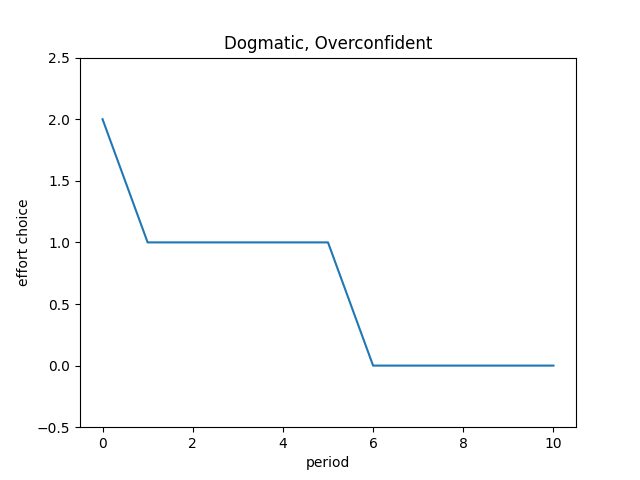
\includegraphics[scale=.5]{dogmatic_over_11.png}
        \caption{$\theta^*=\theta_M$, $\hat\theta=\theta_H$, $\omega^*=\omega_M$}
    \end{figure}
\end{frame}

\begin{frame}{The Switcher (paradigm shifts)}
    Same initial belief as the Dogmatic, but is willing to consider and alternative paradigm $\theta'$\\
    \bigskip
    Keeps track of the likelihoods of the two possible paradigms:\\
    \begin{itemize}
        \item $p_t(s_t|\cdot)$ for $\hat{\theta}$ and $\theta'$
    \end{itemize}
    \bigskip
    They swithch to whichever paradigm is morelikely to have generated the signals
    $$ \frac{p_t(s_t|\theta')}{p_t(s_t|\hat{\theta})}>\alpha\geq1$$
    
\end{frame}


\begin{frame}{The Switcher: Mechanism}
    

    \begin{enumerate}
        \item Chooses $e_H$ and is disappointed $\rightarrow$ adjust belief about $\omega$ downward\\
        \bigskip
        \item Eventually chooses $e_M$ and is disappointed as well $\rightarrow$ adjust belief about $\omega$\\
        \bigskip
        \item Avoids the self-defeating equilibrium if the likelihood of $\theta_M$ becomes larger than that of $\theta_H$
    \end{enumerate}
    
    
\end{frame}

\begin{frame}{Switcher Overconfident: Simulation}
    \begin{figure}
        \centering
        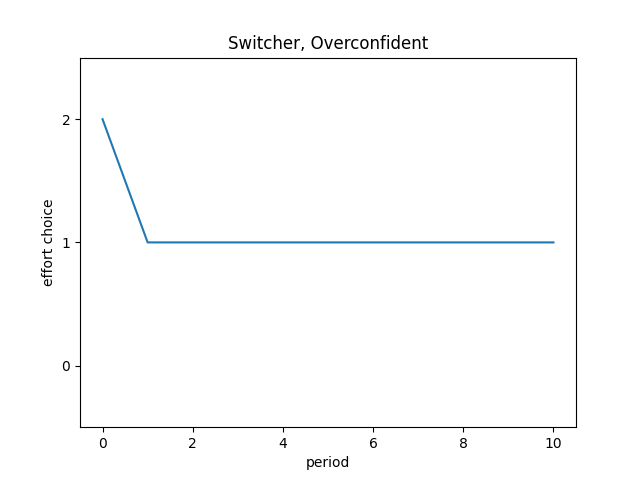
\includegraphics[scale=.5]{switcher_over_11.png}
        \caption{$\theta^*=\theta_M$, $\hat\theta=\theta_H$, $\omega^*=\omega_M$, $\alpha= 1.1$}
    \end{figure}
\end{frame}


\begin{frame}{Self-Attribution Bias / Optimal Expectations}

    Start with a diffused prior over $(\theta, \omega)$ but updates with a bias

    $$ p_{t+1}(\theta, \omega| s_t)=\frac{p_t(s_t|\theta, \omega)^{c(\theta, \omega, s_t)}p_t(\theta, \omega)}{\sum_{(\theta', \omega')}p_t(s_t|\theta', \omega')^{c(\theta', \omega', s_t)}p_t(\theta', \omega')} $$

    Bias is such that 
    $$c(\theta_H, \omega, \text{good news}) \leq c(\theta_M, \omega, \text{good news}) \leq c(\theta_L, \omega, \text{good news})\leq1 \quad \forall \omega$$
    And
    $$c(\theta, \omega_L, \text{bad news}) \leq c(\theta, \omega_M, \text{bad news}) \leq c(\theta, \omega_H, \text{bad news})\leq1 \quad \forall \theta$$
    

\end{frame}

\begin{frame}{Self-Attribution: Mechanism}
    \begin{enumerate}
        \item Chooses $e$ that maximizes utility according to priors
        \bigskip
        \begin{itemize}
            \item Belief on $\mathbb{E}[\omega]$ deteriorates a lot after bad news $\to$ big change in effort
            \item Belief on $\mathbb{E}[\theta]$ increases a lot after good news $\to$ small positive (or negative) change in effort \\
        \end{itemize}
    \end{enumerate}
    
\end{frame}


\begin{frame}{Self-Attribution: Simulation}
        \begin{figure}
            \centering
            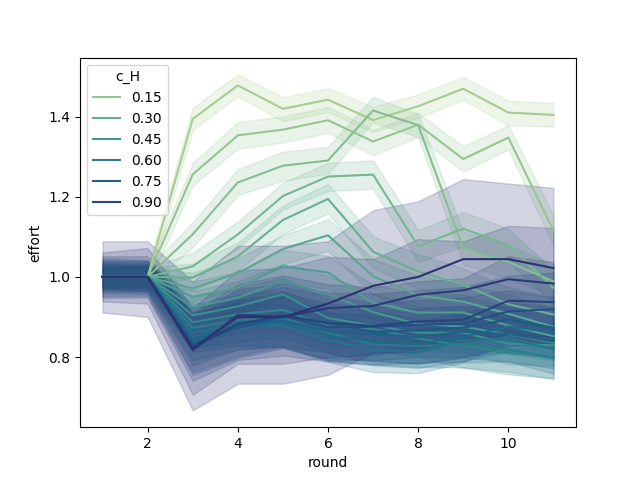
\includegraphics[scale=.5]{self-serving_11.png}
        
        \end{figure}
    \end{frame}

    \begin{frame}{Myopic Bayesian}

        Start with a diffused prior over $(\theta, \omega)$ and updates correctly
    
        $$ p_{t+1}(\theta, \omega| s_t)=\frac{p_t(s_t|\theta, \omega)p_t(\theta, \omega)}{\sum_{(\theta', \omega')}p_t(s_t|\theta', \omega')p_t(\theta', \omega')} $$
    
        But if they start with a prior that is ``tight" 
        around a self-defeating equilibrium they will never learn 
        
    \end{frame}


    \begin{frame}{All Models}
    \label{Figure2}
        \begin{figure}
        \centering
        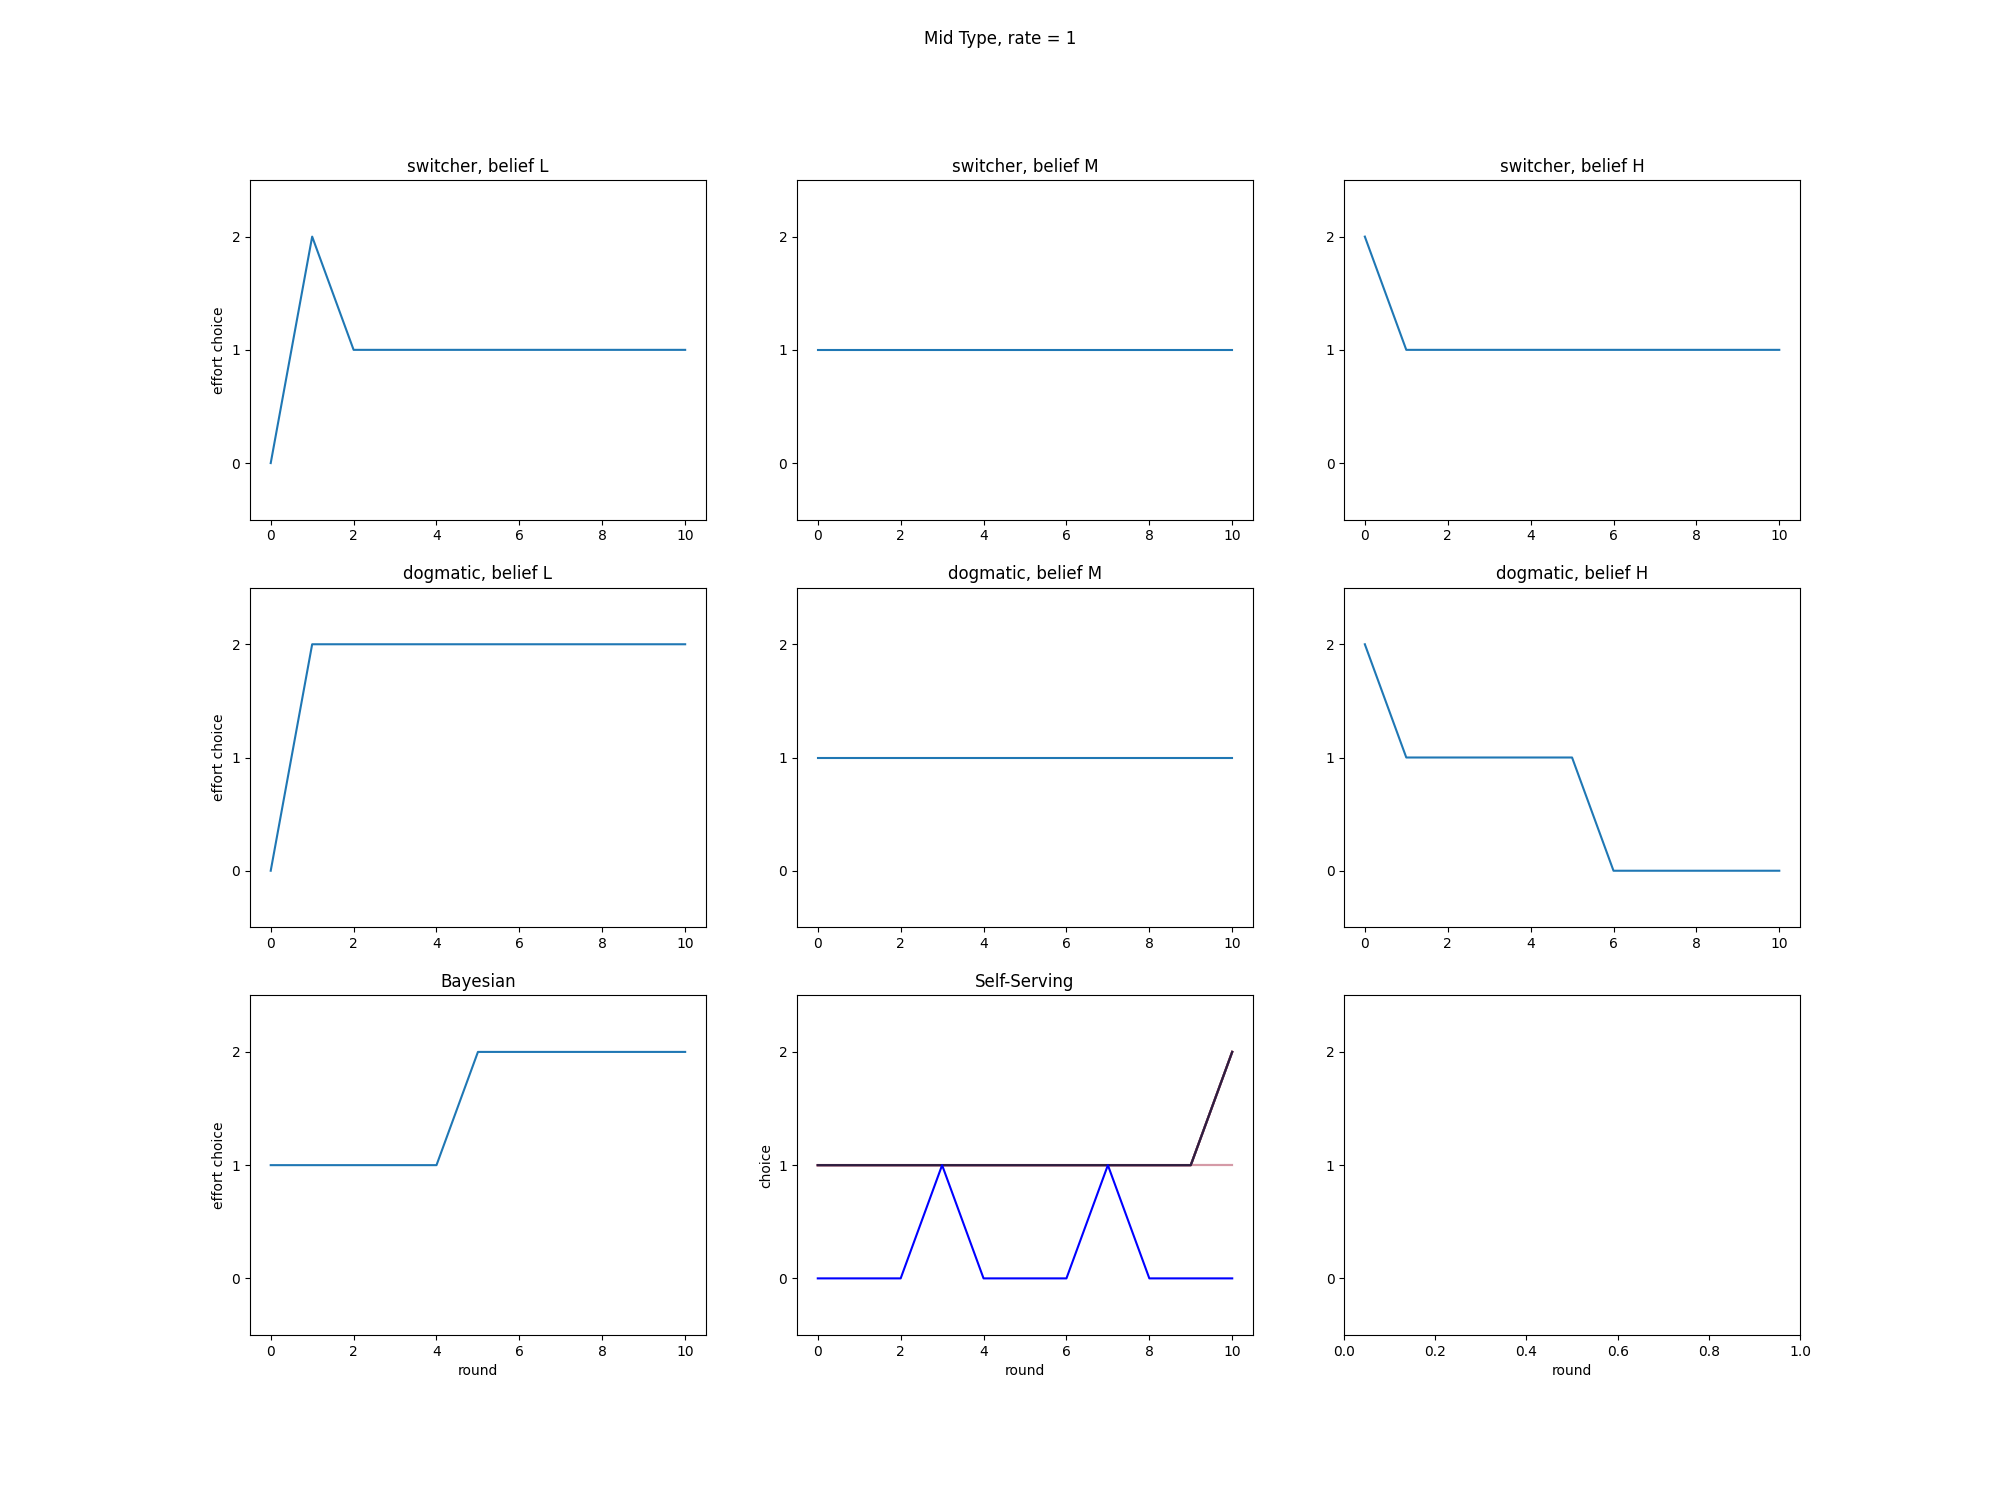
\includegraphics[scale=0.2]{all_11.png}
    \end{figure}     

\end{frame}



\section*{Experimental Design}

\begin{frame}{Set the Types}
    \bigskip
    \begin{itemize}
        \item Quiz: Answer as many questions as you can in 2 minutes\\
        \begin{itemize}
            \item Math, Verbal, Pop-Culture, Science, Us Geography, Sports and Video games\\
        \end{itemize}
        \bigskip

        \item How many questions do you think you answered correctly in each quiz?\\
        \begin{itemize}
            \item 0 to 5 ($\theta_L$)
            \item 6 to 15 ($\theta_M$)
            \item 16 or more ($\theta_H$)
        \end{itemize}
        \item How sure are you about your guess?
        \begin{itemize}
            \item Random guess $\to 1/3$
            \item Another is equally likely $\to 1/2$
            \item Fairly certain $\to 3/4$
            \item Completely sure $\to 1$
        \end{itemize}
    \end{itemize}

\end{frame}


\begin{frame}{Choice and Update}
    Effort choice and feedback (One topic at a time)\\
    \bigskip
    \begin{itemize}
        \item Choose a gamble: A, B or C (effort)
        \item Receive a sample of 10 signal realizations
    \end{itemize}
    \bigskip
    x 11 per topic

\end{frame}

\begin{frame}{Stereotype condition}

    Observe the characteristics of a participant \\
    \begin{itemize}
        \item Gender, 
        \item US National or not \\
    \end{itemize}
    \bigskip
    Answer the same questions about slef and other\\

    \bigskip
    Belief updating and effort choice:\\
    \begin{itemize}
        \item  The DGP depends on the $\theta$ the other participant
    \end{itemize}
    \bigskip
    x 11 per topic

\end{frame}

\begin{frame}{Eliciting Beliefs?}
    \begin{itemize}

        \item $E[\omega]$ is revealed by their choice of effort\\
        \bigskip
        \item Eliciting beliefs for $\theta$ can incentivize learning in a way that is not consistent with the theory\\
        \bigskip
        
    \end{itemize}

    Allow them to see the success rate matrix for only one type. 
    \begin{itemize}
        \item Track the matrices they choose to see in each round
    \end{itemize}

\end{frame}


\begin{frame}{Screen}
    \begin{figure}
        \centering
        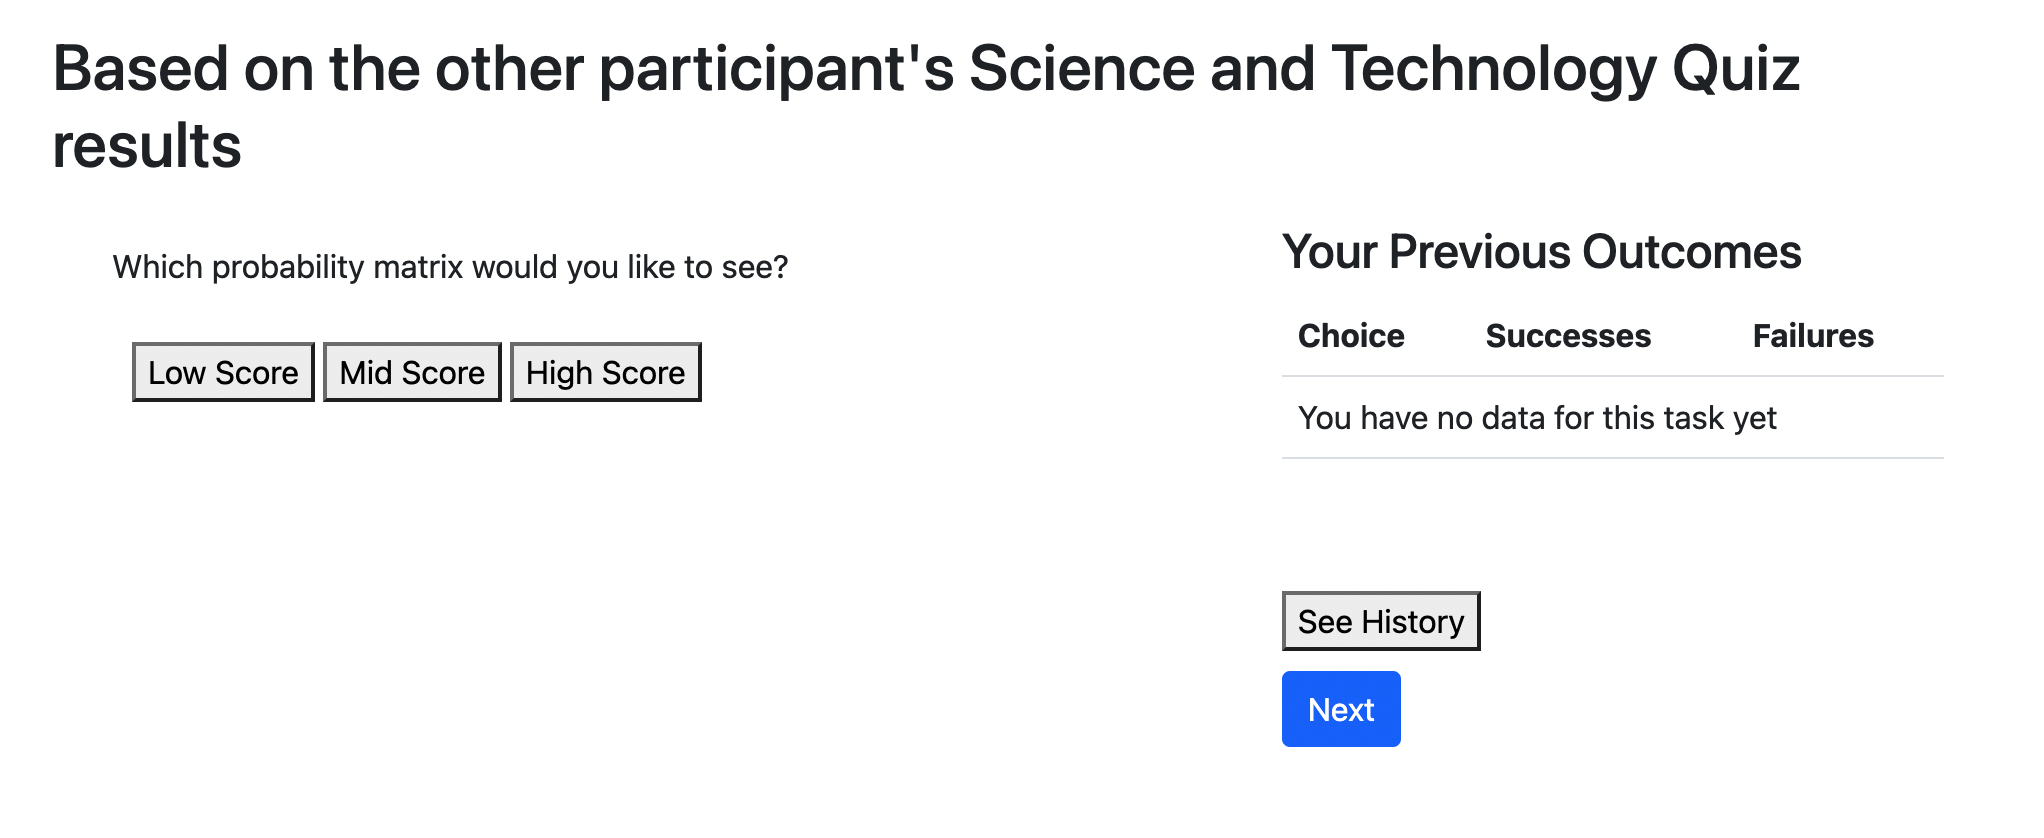
\includegraphics[scale=.4]{screen1.png}
    \end{figure}
\end{frame}

\begin{frame}{Screen}
    \begin{figure}
        \centering
        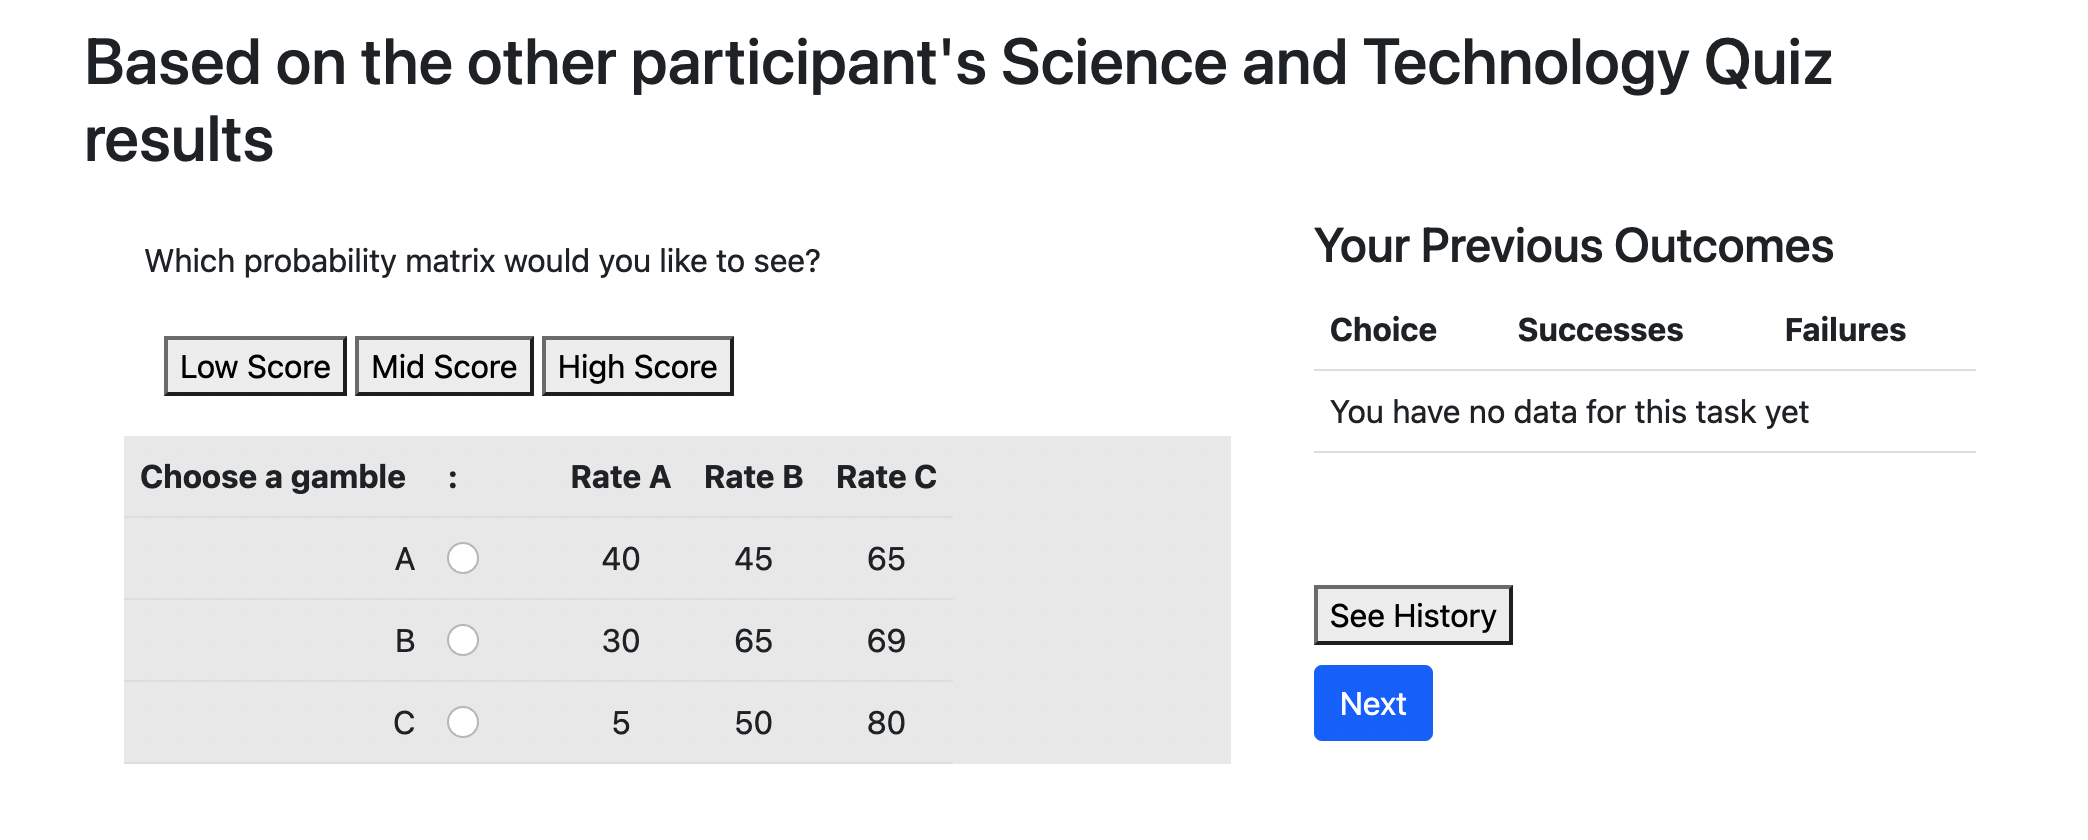
\includegraphics[scale=.4]{screen2.png}
    \end{figure}
\end{frame}

\section*{The Data}

\begin{frame}{The Data}
    Subject pool:\\
    \begin{itemize}
        \item Run at the CESS lab in person
        \item 45 subjects in Ego
        \item 33 subjects in Stereotype
    \end{itemize}
    \bigskip
    The Sessions:
    \begin{itemize}
        \item 8 sessions 
        \item 45 minutes on average
        \item Average payment: $\$23$
        \begin{itemize}
            \item $\$10$ show-up fee
            \item $\$ 0.20$ per correct answer
            \item $\$ 0.20$ per success
            \item Paid one topic at random
        \end{itemize}
    \end{itemize}
    
\end{frame}

\begin{frame}{Initial Misspecifications}
    \label{initialhist}
    \begin{figure}
        \centering
        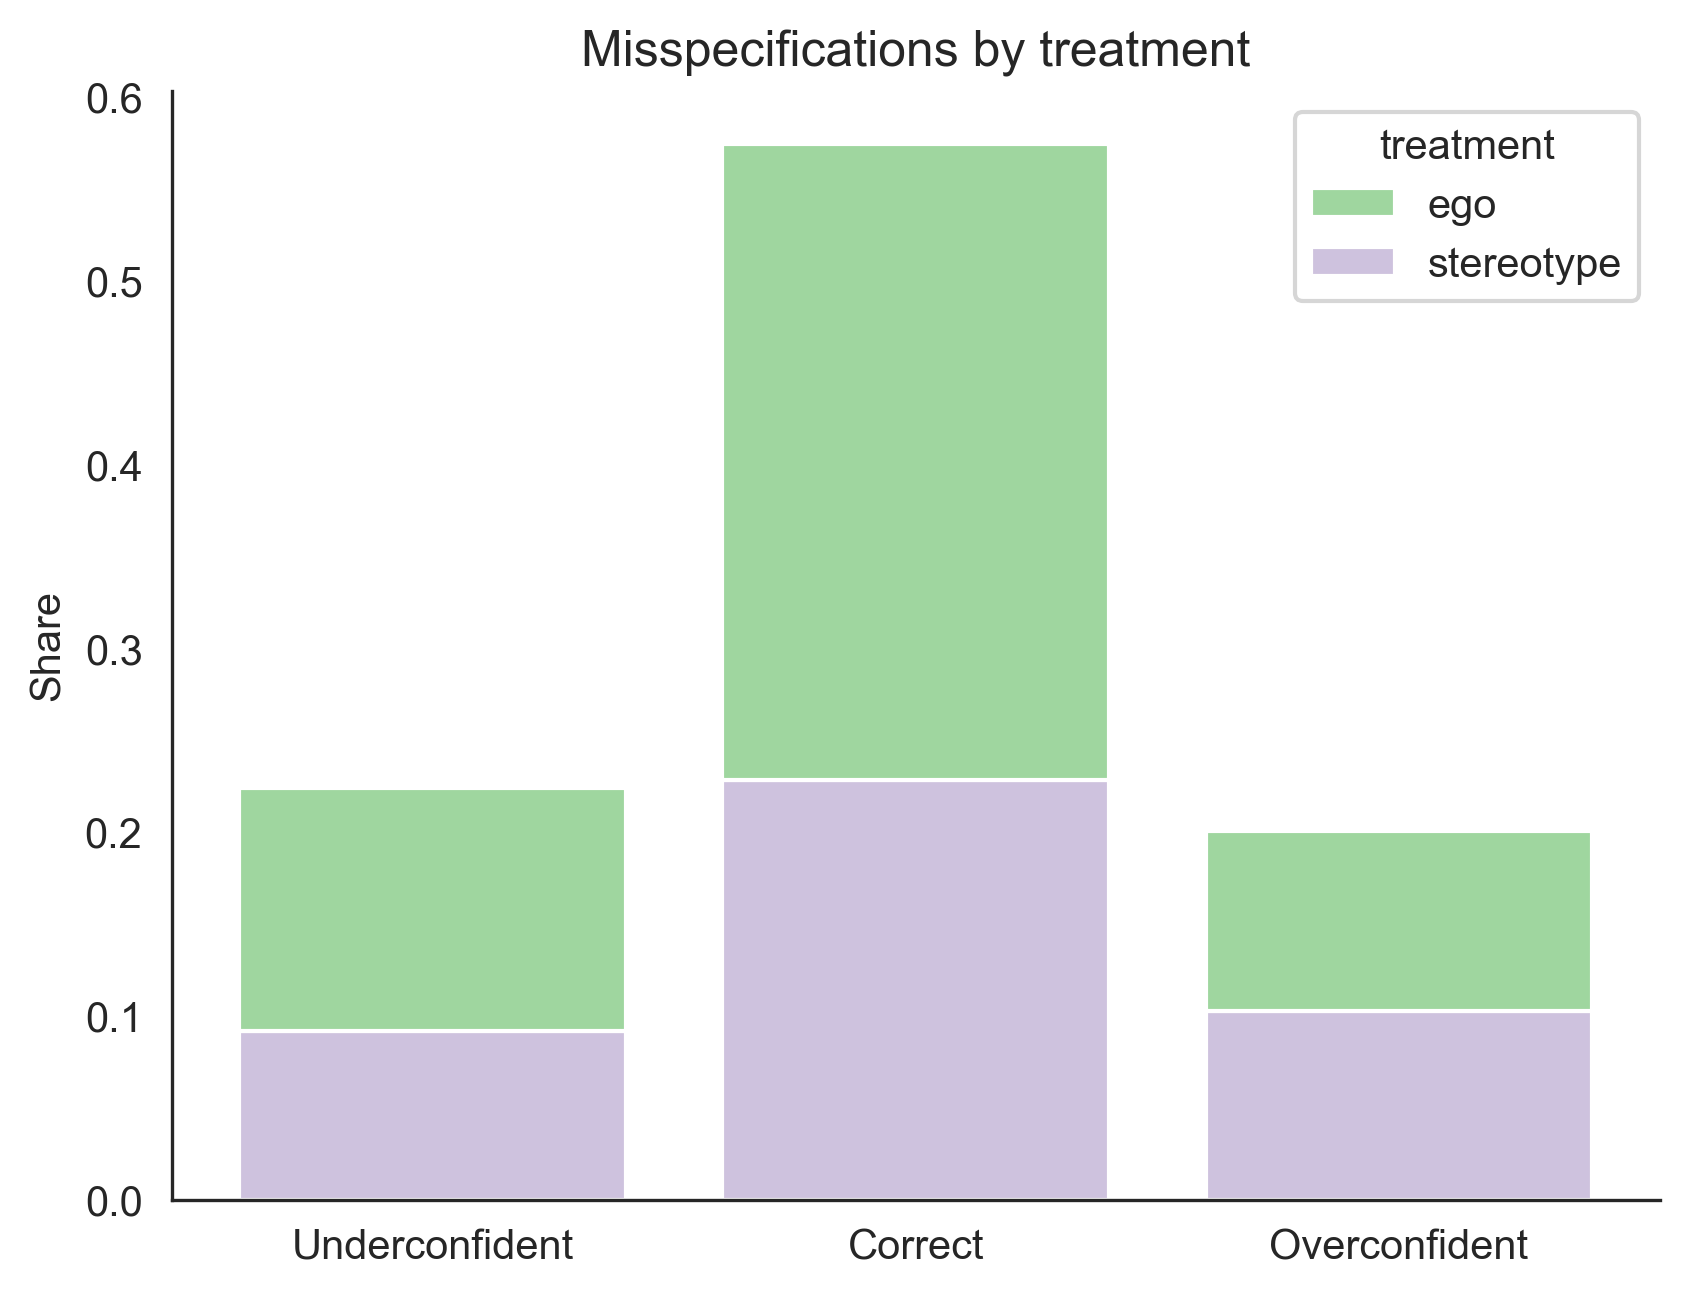
\includegraphics[scale=.5]{misspecification_hist.png}
    \end{figure}
    \action{\hyperlink{certainties}{\beamerbutton{certainties}}}

\end{frame}

\begin{frame}{The Stereotypes}
    \label{typeheat}
    \begin{figure}
        \centering
        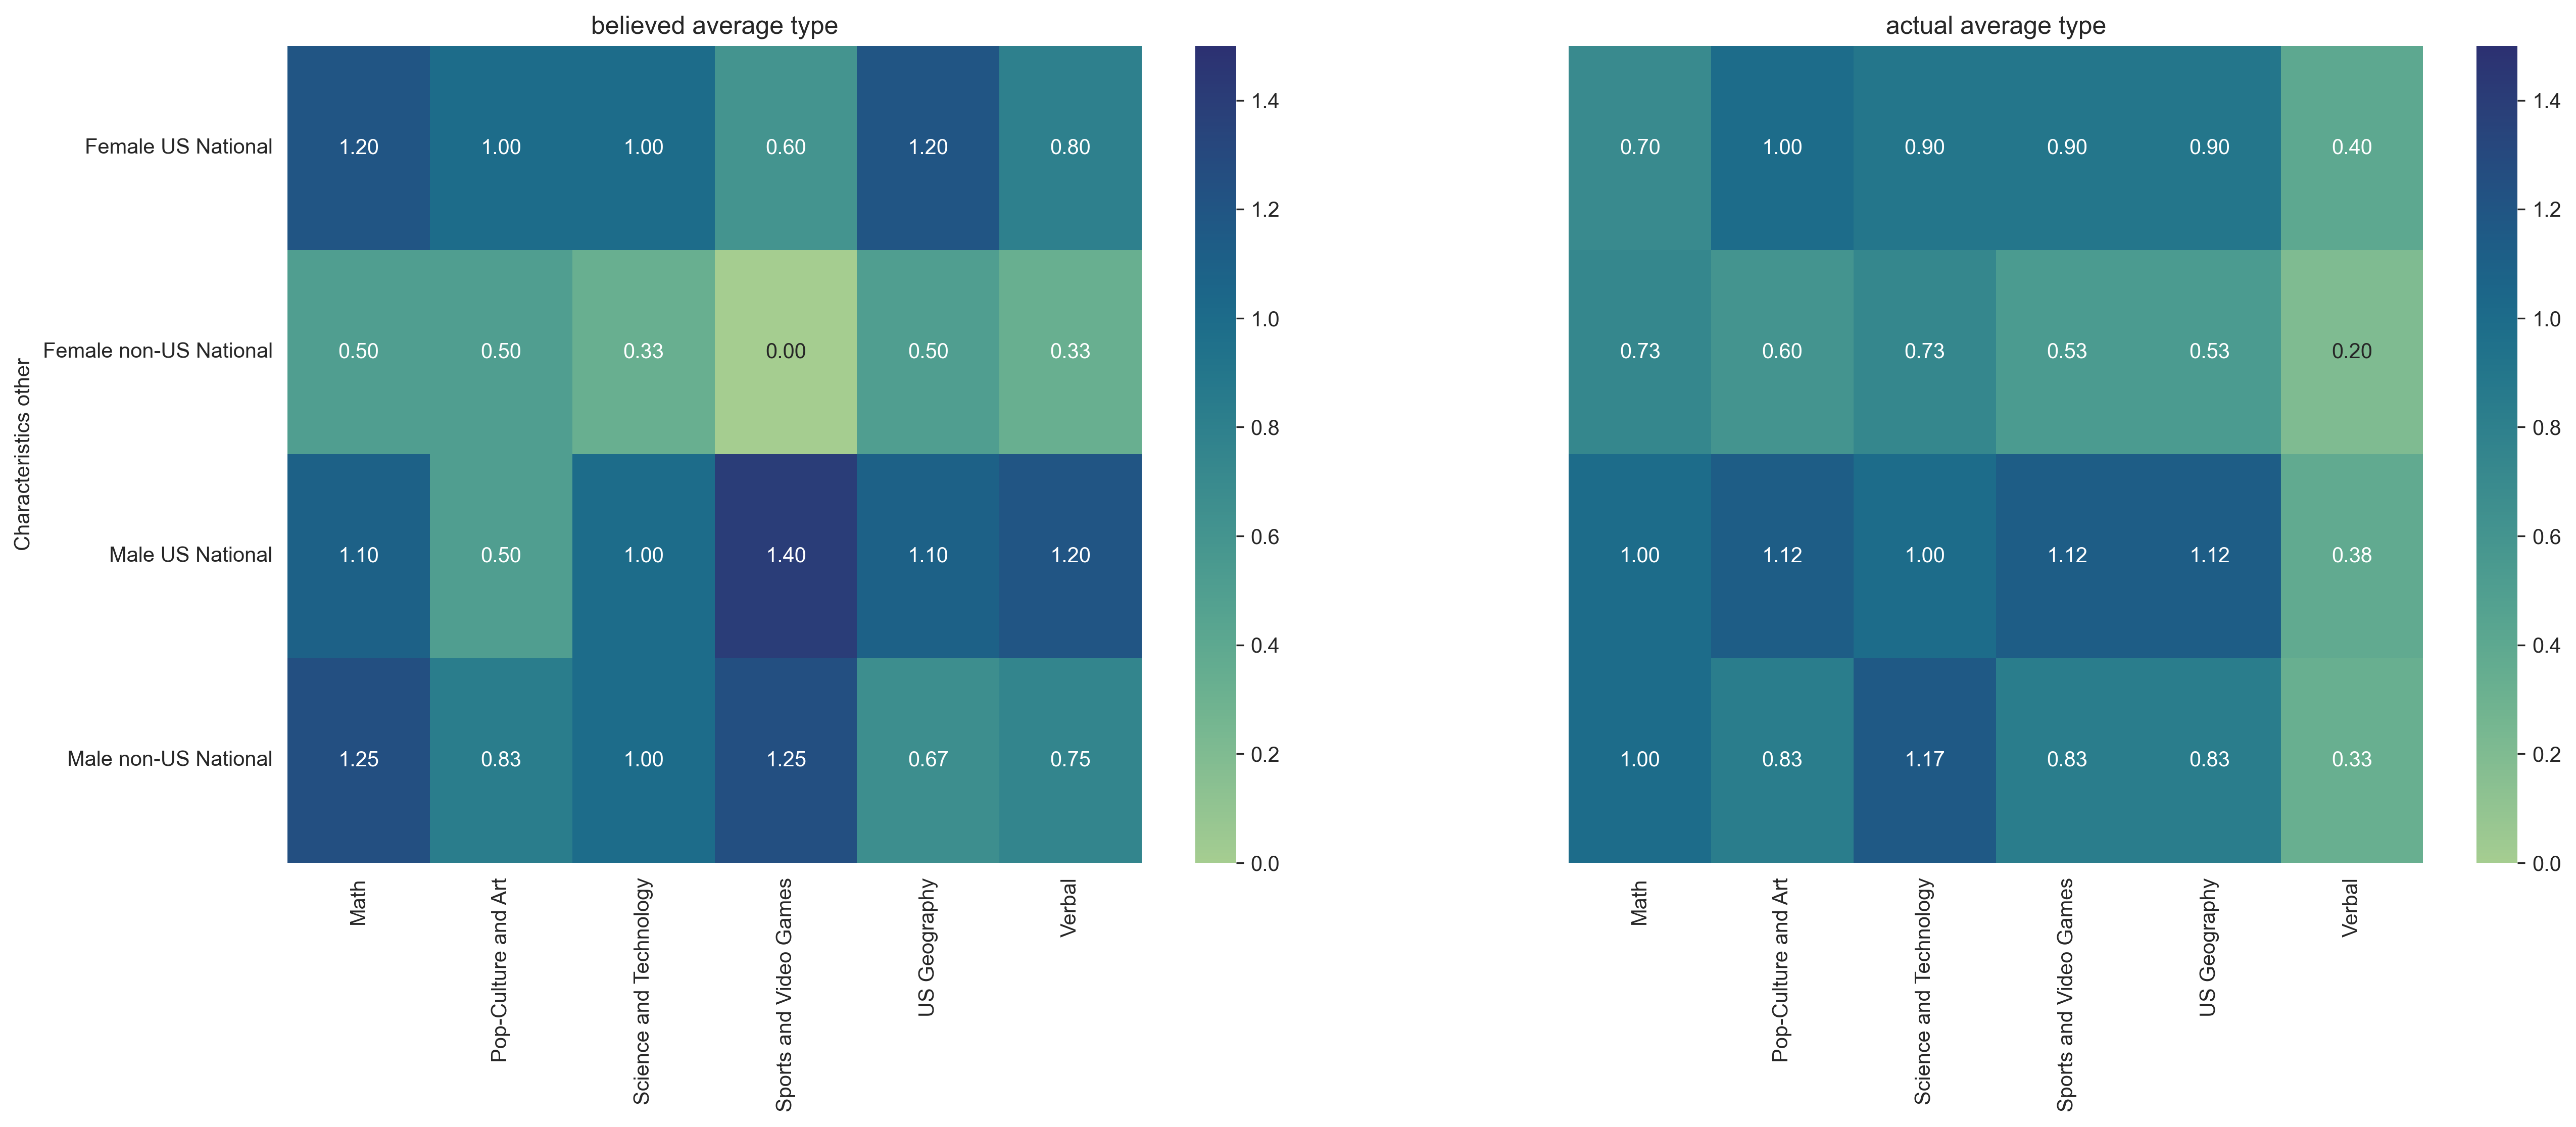
\includegraphics[scale=.3]{believed_actual_type_heat.png}
    \end{figure}

    %add a hyperlink button to the appendix slide with the misspecification_heat
    \action{\hyperlink{misspecificationsheat}{\beamerbutton{misspecifications}}} 

\end{frame}


\begin{frame}{Learning $\omega$}
    \begin{figure}
        \centering
        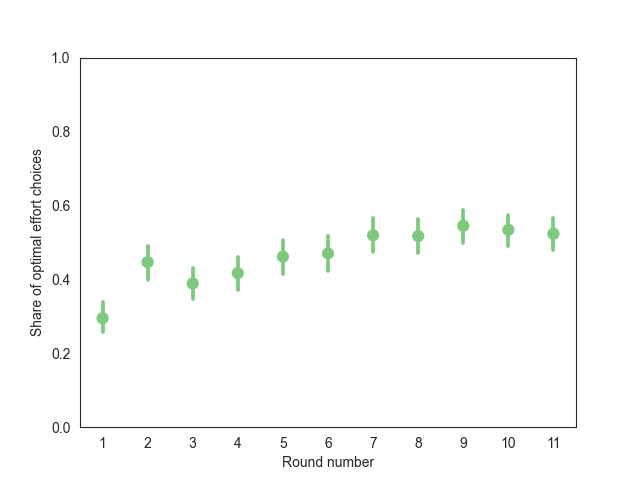
\includegraphics[scale=.5]{effort_learning.png}
    \end{figure}

\end{frame}

\begin{frame}{Learning $\Theta$}
    \begin{figure}
        \centering
        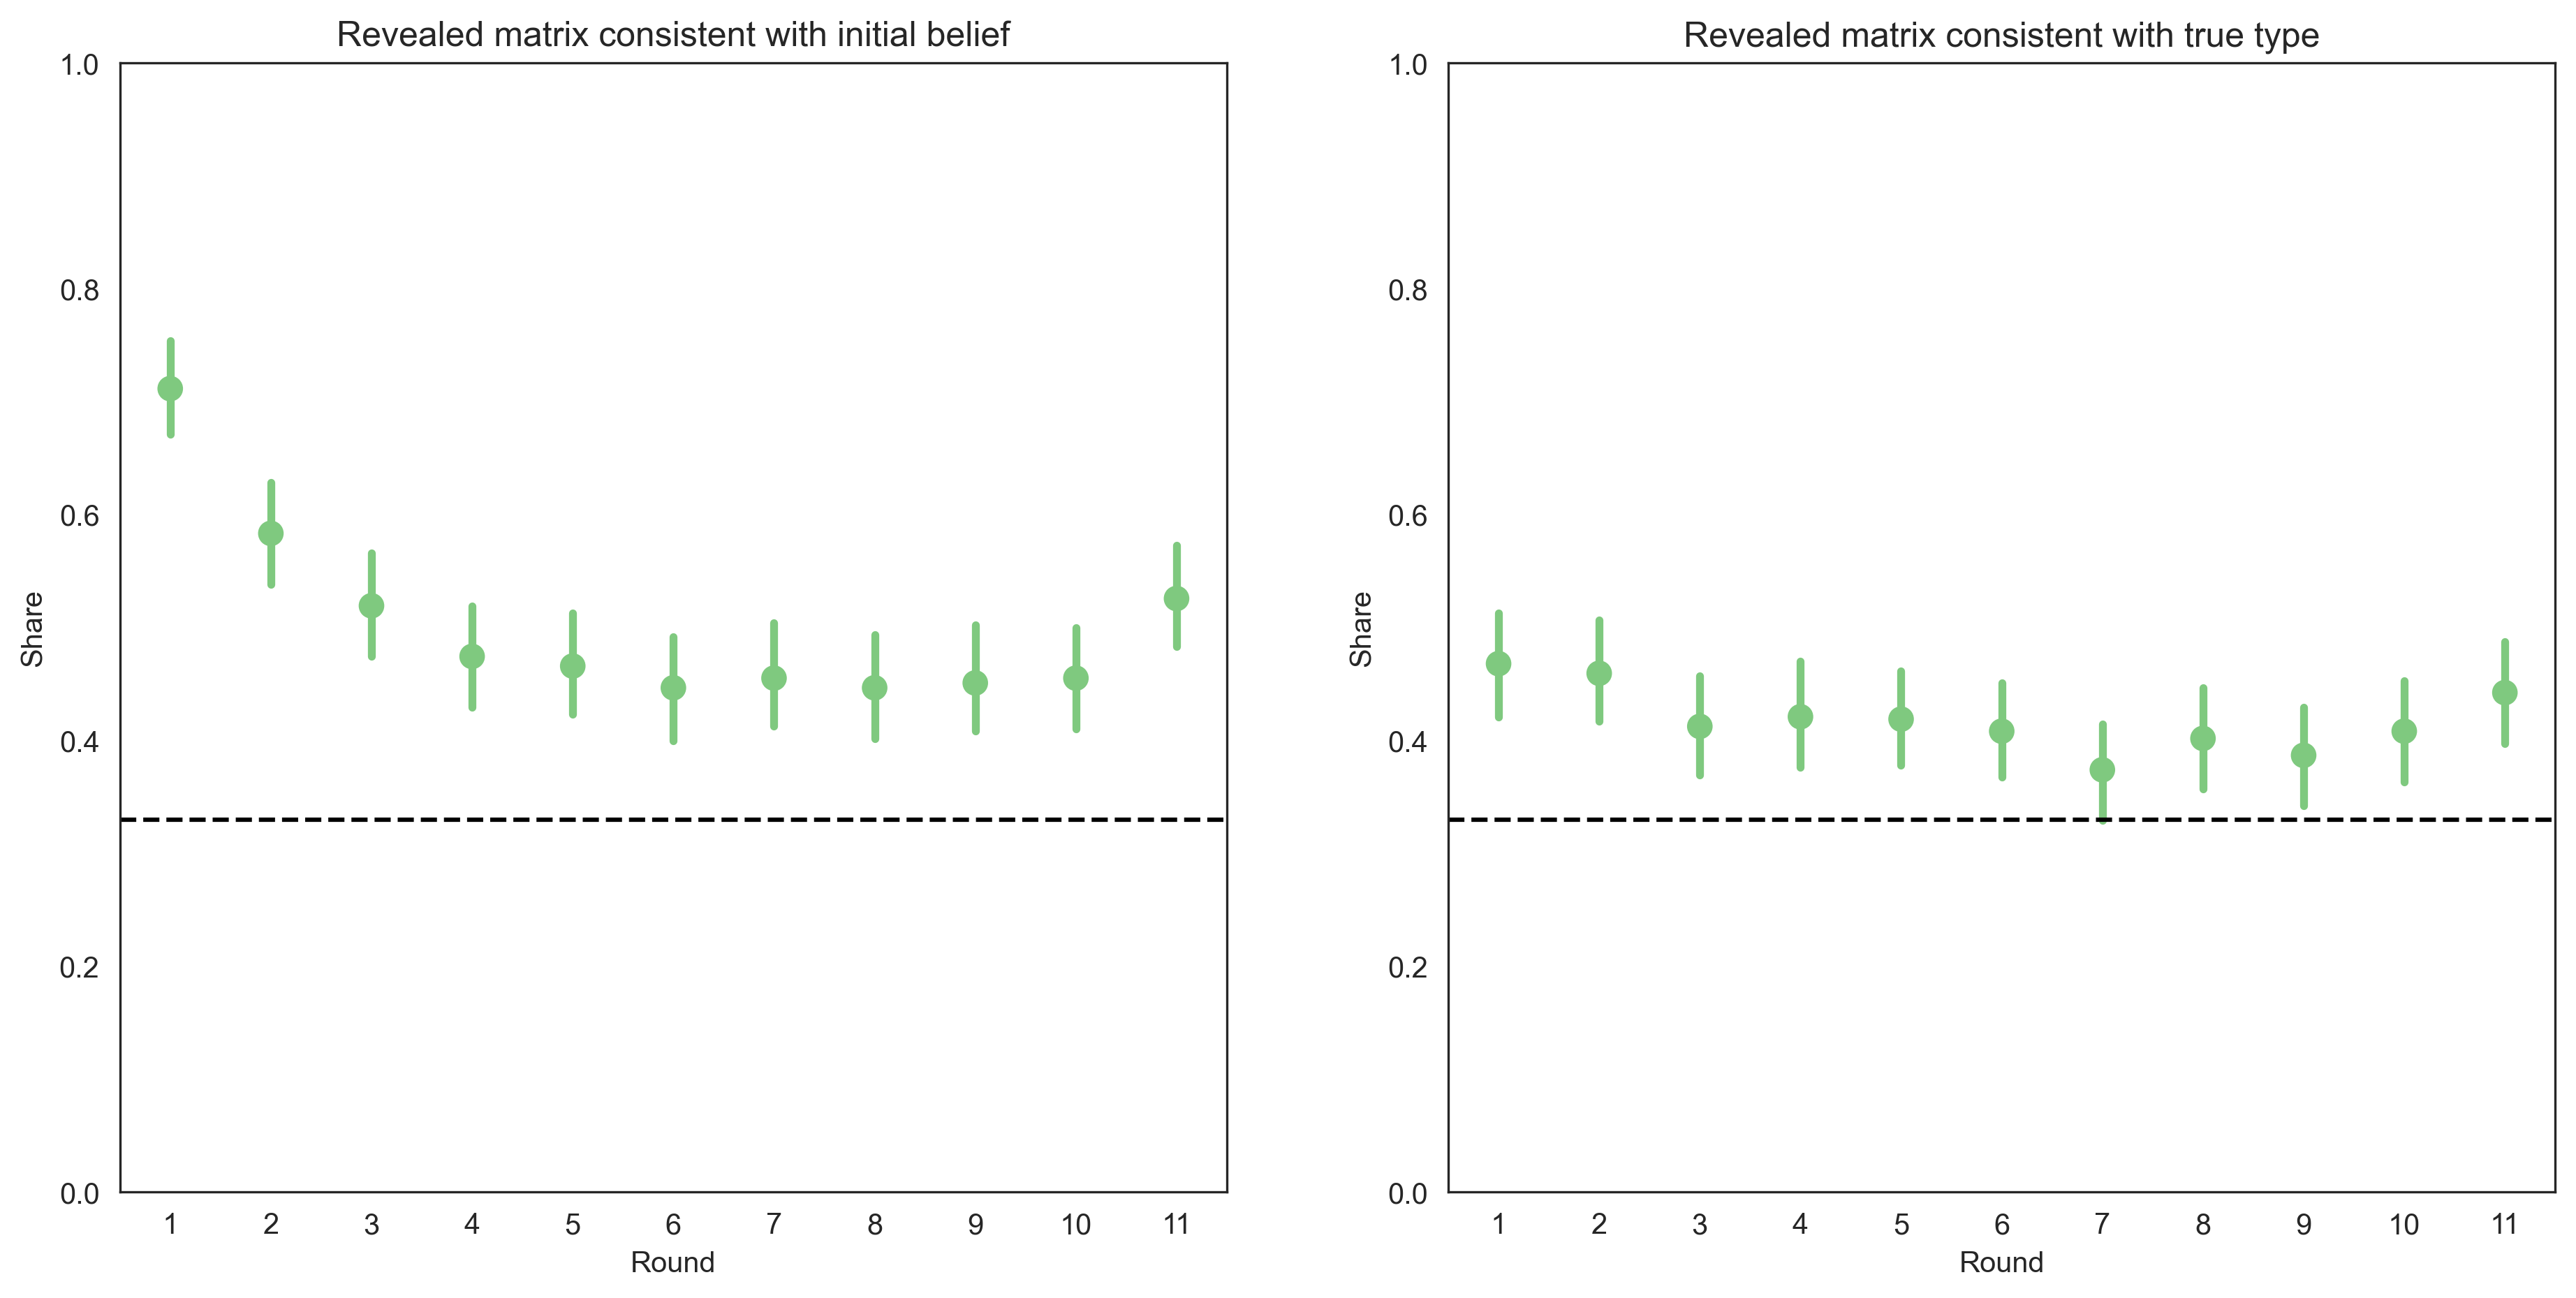
\includegraphics[scale=.33]{last_button_consistency.png}
    \end{figure}
    
\end{frame}

\begin{frame}{Changes in Misspecifications}
    \label{misspecificationsroundstypes}
    \begin{figure}
        \centering
        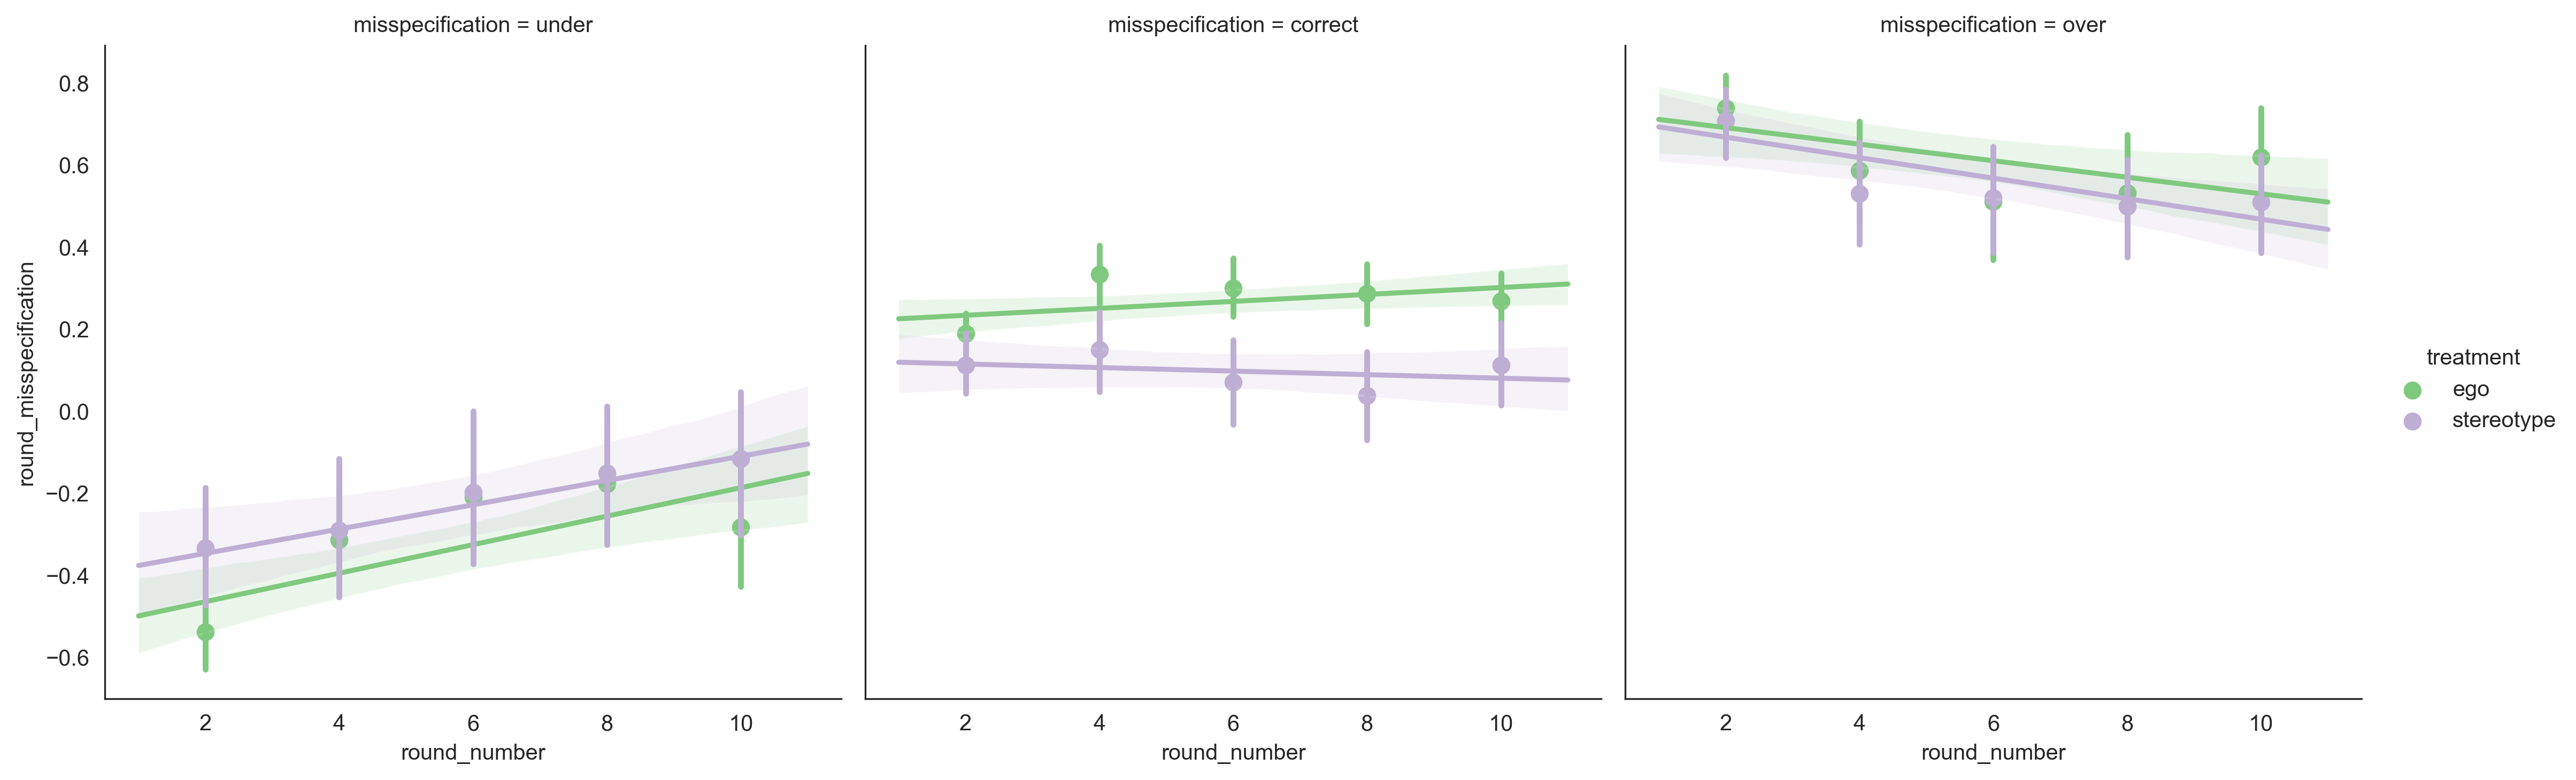
\includegraphics[scale=.3]{misspecification_evolution_tratment.png}
    \end{figure}
    \action{\hyperlink{misspecificationsrounds}{\beamerbutton{overall}}}
\end{frame}

\begin{frame}{Transitions}
    \begin{figure}
        \centering
        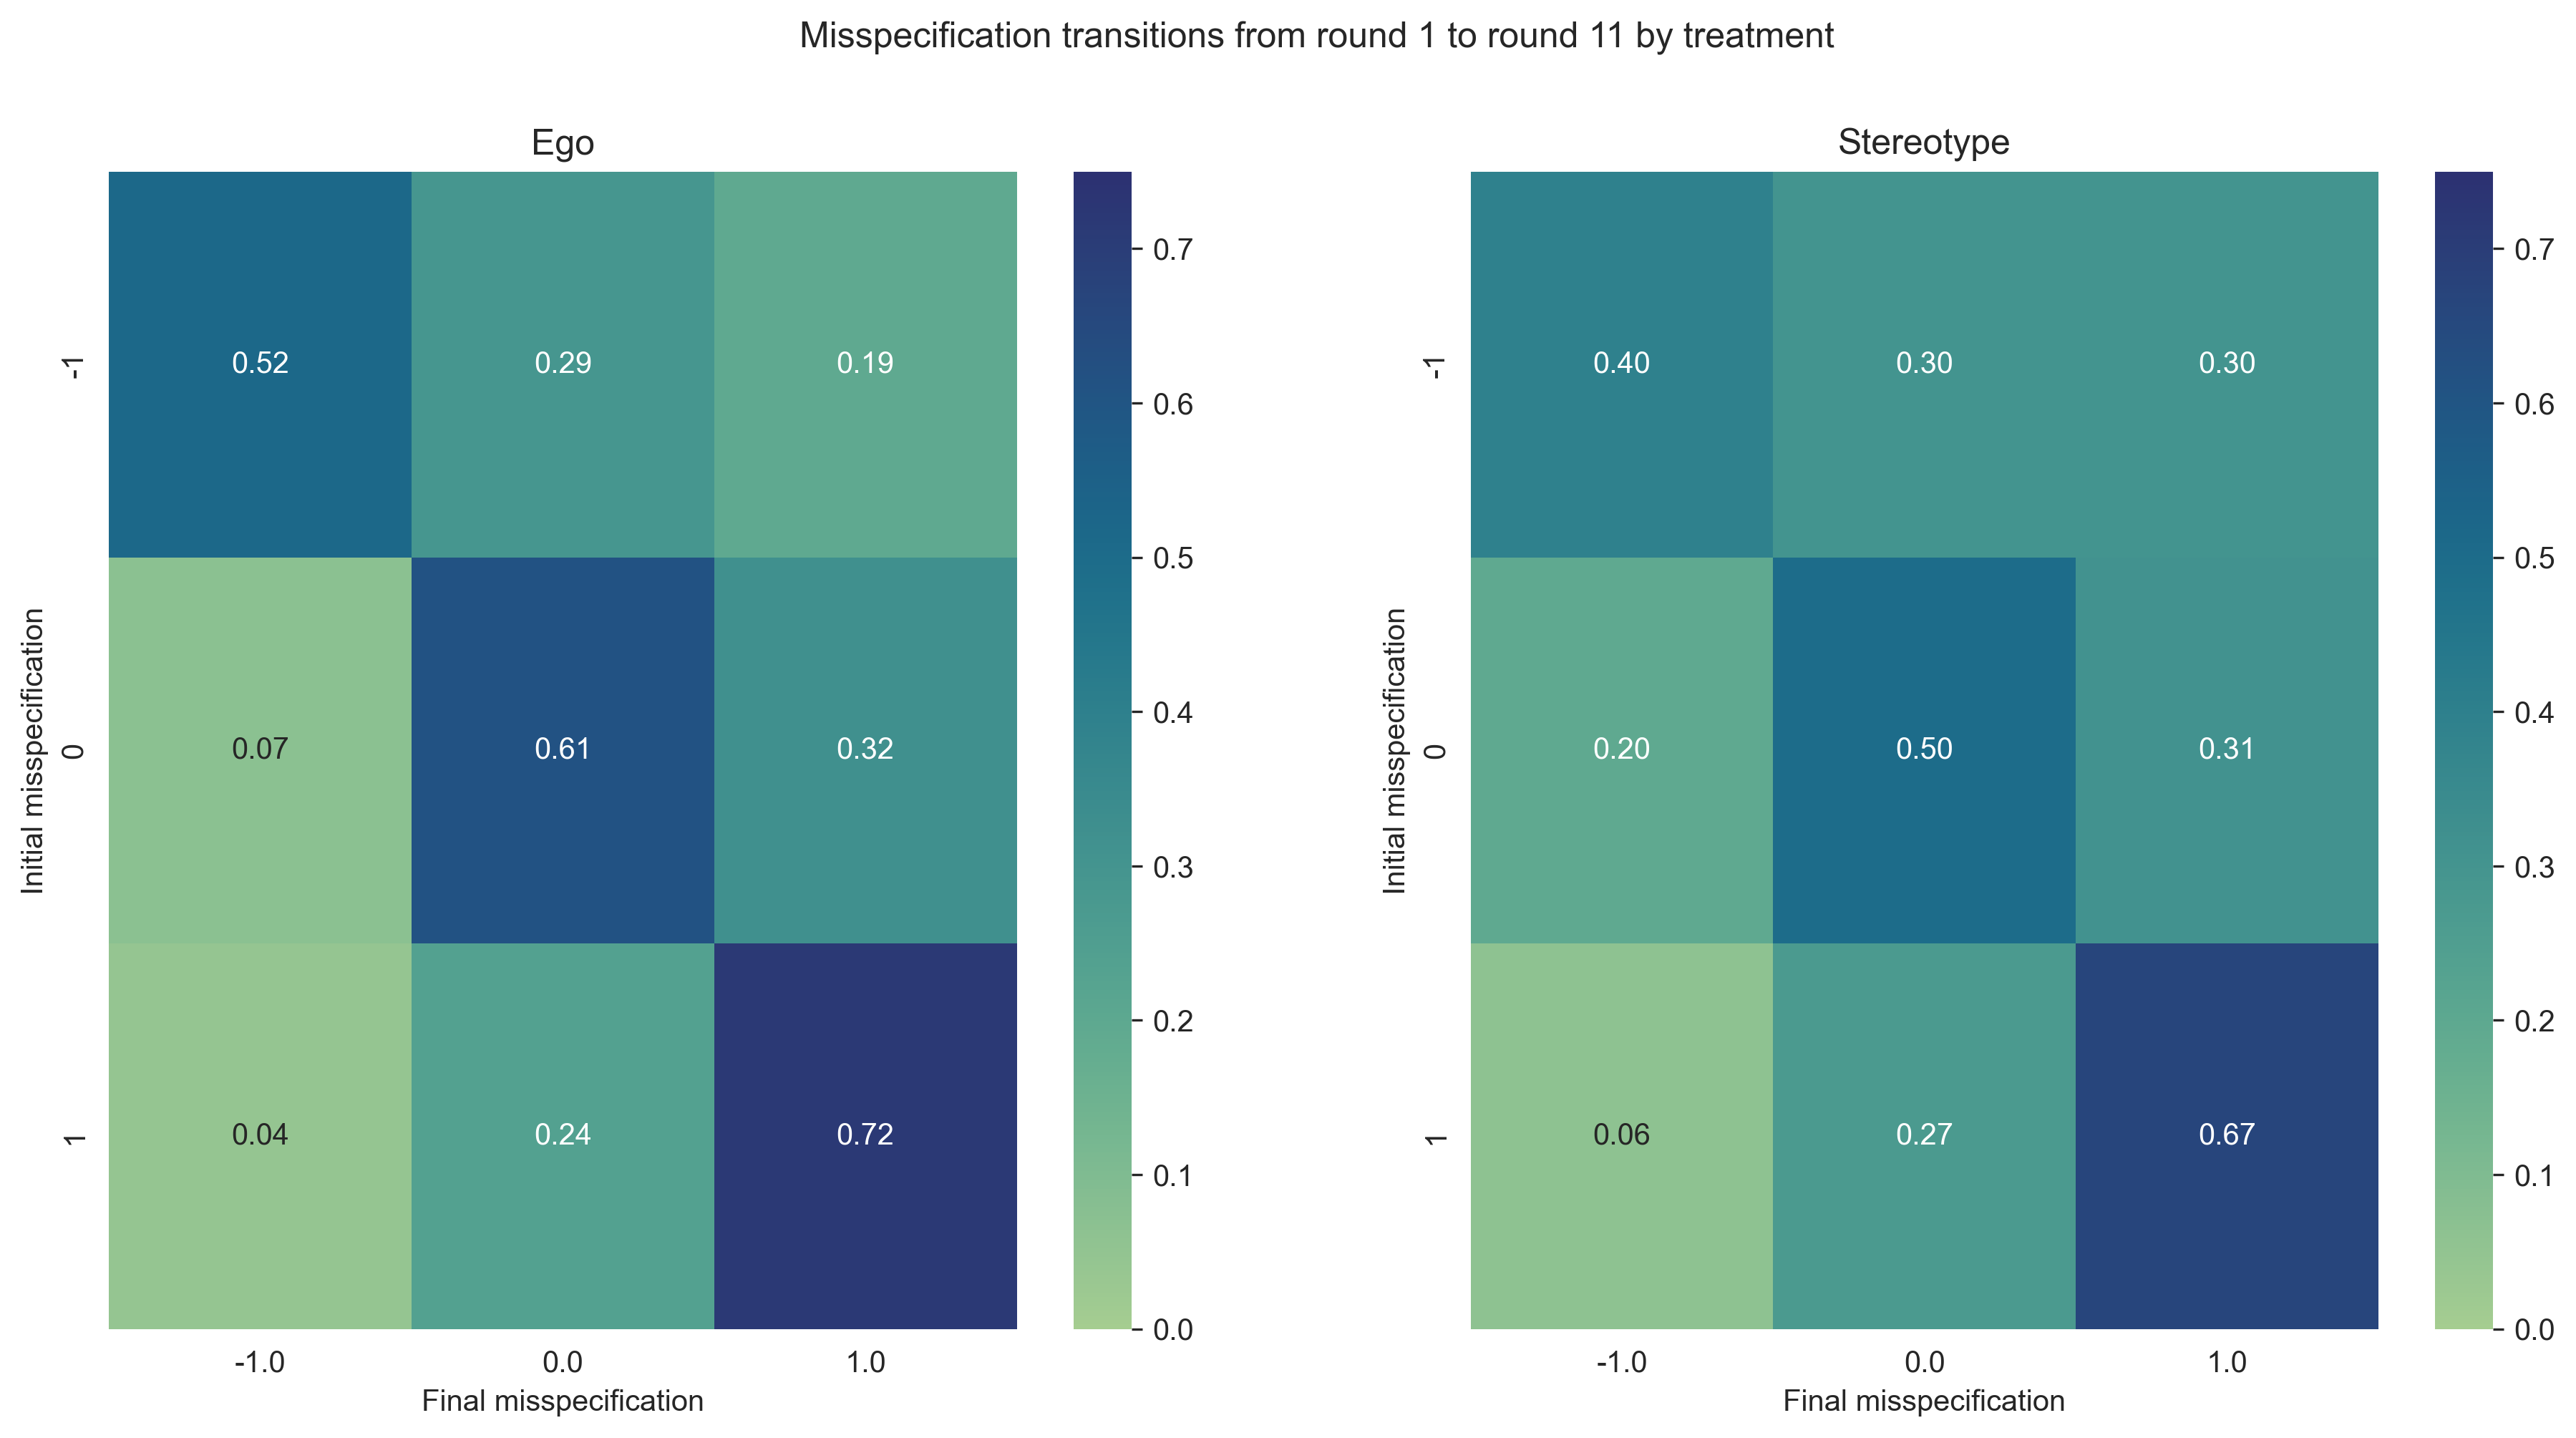
\includegraphics[scale=.35]{misspecification_transitions_treatment.png}
    \end{figure}
    
\end{frame}

\begin{frame}{Good News v. Bad News}
    \label{goodvbad}
    \begin{figure}
        \centering
        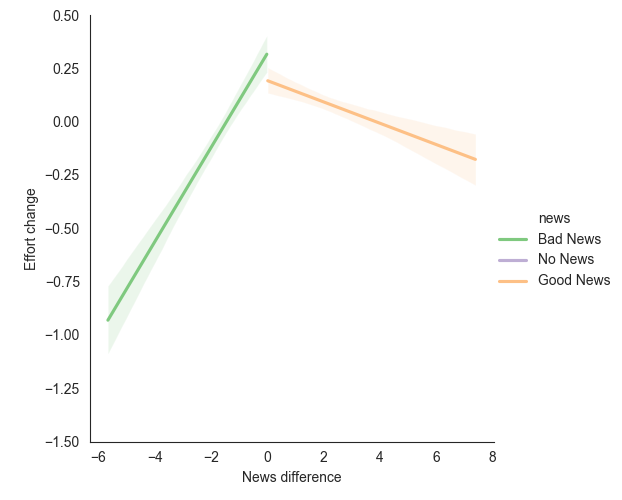
\includegraphics[scale=.5]{effort_change_news.png}
    \end{figure}
    \action{\hyperlink{positivevnegative}{\beamerbutton{other}}}

\end{frame}

\section*{Parameters}

\begin{frame}{Identification of $\alpha$}

    Whenever the agent switches from one paradigm to another, they are revealing that \\
    $$\frac{p_t(s^t|\theta')}{p_t(s^t|\hat{\theta})}=\alpha$$

    \bigskip
    Notice that this identifies an upper bound for $\alpha$\\
    \bigskip

    I take the average value of the likelihood ratio when the agent changes their choice of $\theta$
    to be $\alpha $\\
    \bigskip
    I find $\alpha=1.48$ and no difference across treatments\\


\end{frame}

\begin{frame}{Calibration of Bias}
    
    Simulation on a grid of parameters\\
    \bigskip
    For each task take the parameters that minimize the distance between the simulated and the actual effort\\
    \bigskip
    Average for each subject\\
    \bigskip
    Average across subjects\\
    
    \begin{align*}
        c(\theta_H, \omega, \text{good news}) & =  c(\theta, \omega_L, \text{bad news})= 0.137\\
        c(\theta_M, \omega, \text{good news}) & =  c(\theta, \omega_M, \text{bad news}) = 0.36\\
        c(\theta_L, \omega, \text{good news}) & =  c(\theta, \omega_H, \text{bad news}) = 1
    \end{align*}
    
\end{frame}

\section*{Heterogeneity}

\begin{frame}{Model Fit: Distributions}

    \begin{figure}
        \centering
        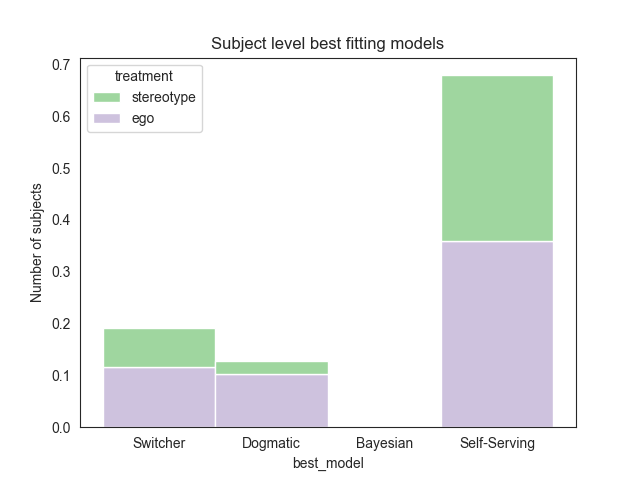
\includegraphics[scale=.5]{model_fit_histogram.png}
    \end{figure}
    
\end{frame}

\begin{frame}{Model Fit: Distance}
    \label{meandistances}
    \begin{figure}
        \centering
        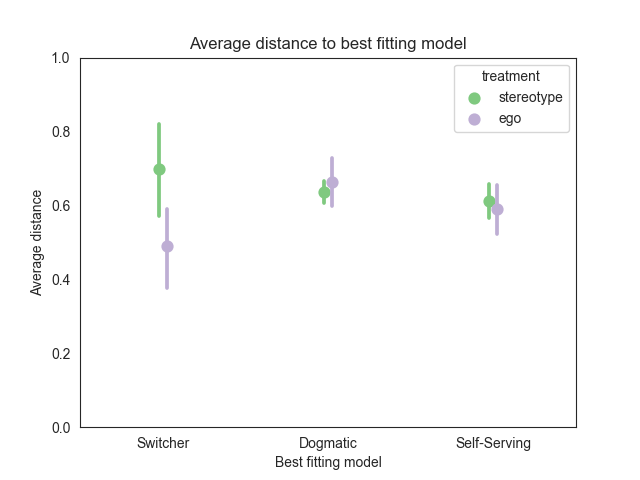
\includegraphics[scale=.5]{model_min_distance.png}
    \end{figure}

    \action{\hyperlink{pathdistances}{\beamerbutton{paths}}}
    
\end{frame}

\section*{Concluding Remarks}

\begin{frame}{Summary}

\begin{itemize}
    \item Data is not fully consistent with the models
    \item Some indications of self-attribution bias and/or paradigm shifts
    \item Need a better estimation of the parameters
    \item Are subjects experimenting in order to learn?
    \begin{itemize}
        \item Hestermann and Le Yaouanq (2021)
    \end{itemize}
\end{itemize}
    
\end{frame}

\begin{frame}{What is Next}
    \begin{enumerate}
        \item Have a better estimation of the attribution bias parameters
        \begin{itemize}
            \item Estimate using SMM
            \item Elicit beliefs within this framework
        \end{itemize}
        \item Can dynamic learning explain the data better?
        \begin{itemize}
            \item This model would predict underconfidence to be more persistent than overconfidence
        \end{itemize}

    \end{enumerate}
    
\end{frame}


\begin{frame}{The end}
    \large\textbf{Thank you!}
\end{frame}

\appendix

\begin{frame}{Misspecifications}
    \label{misspecificationsheat}
    \begin{figure}
        \centering
        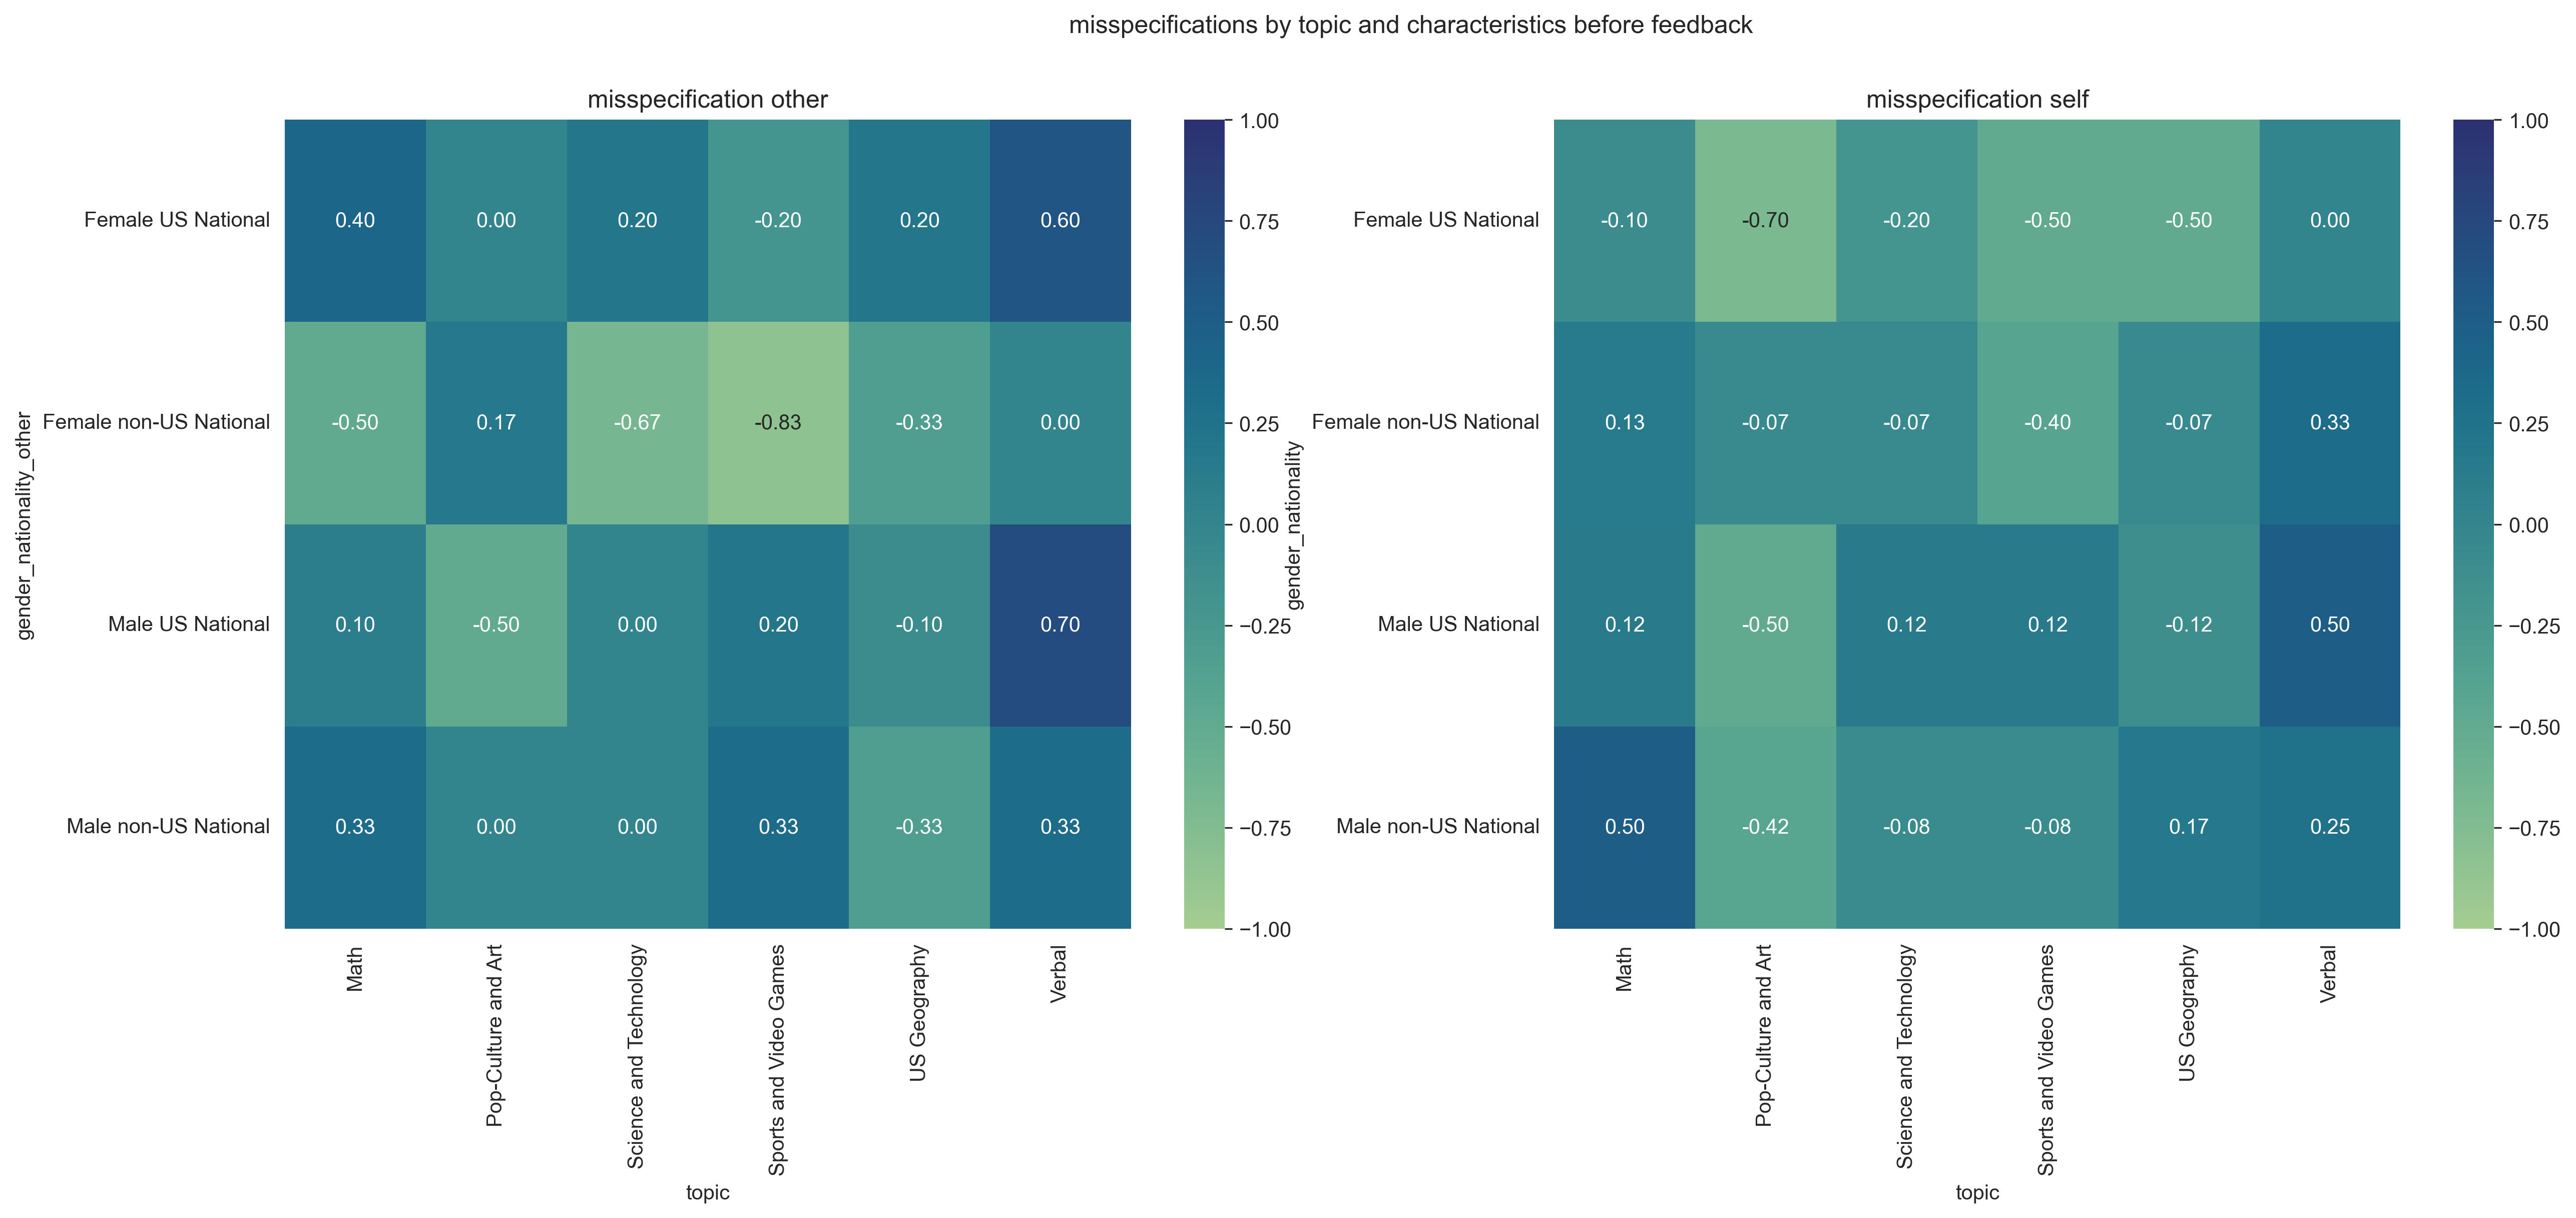
\includegraphics[scale=.3]{misspecifications_characteristics_treatment.png}
    \end{figure}
    \action{\hyperlink{typeheat}{\beamerbutton{Back}}}
\end{frame}

\begin{frame}{Certainties}
    \label{certainties}
    \begin{figure}
        \centering
        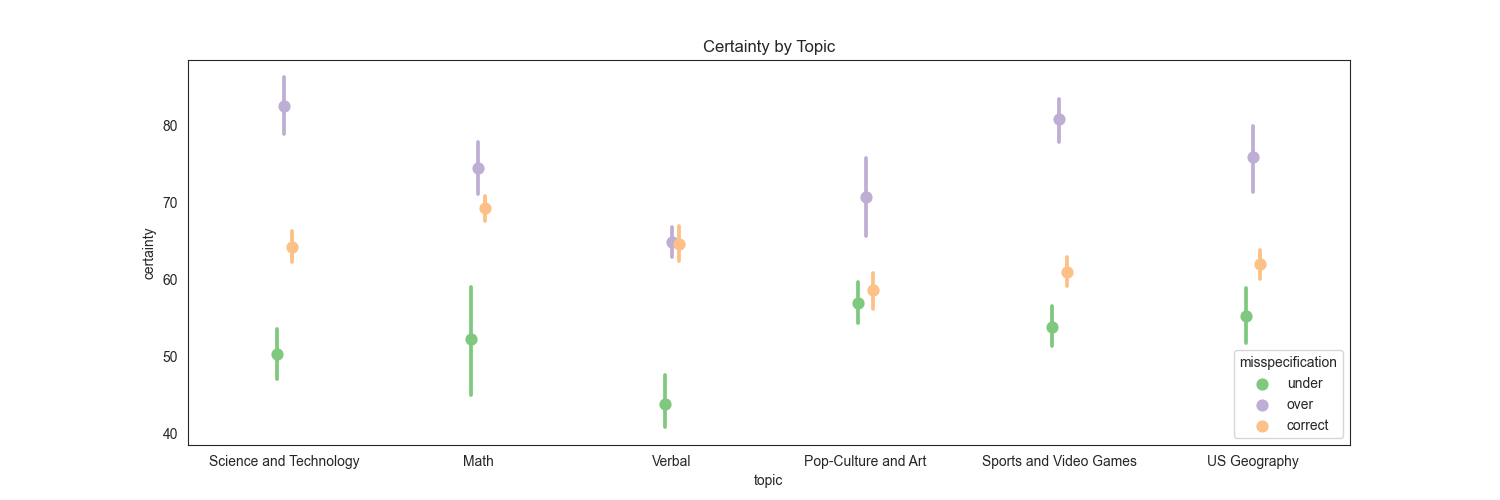
\includegraphics[scale=.4]{certainty_by_topic.png}
    \end{figure}

    \action{\hyperlink{initialhist}{\beamerbutton{Back}}}
\end{frame}

\begin{frame}{Misspecification changes by treatment}
    \label{misspecificationsrounds}
    \begin{figure}
        \centering
        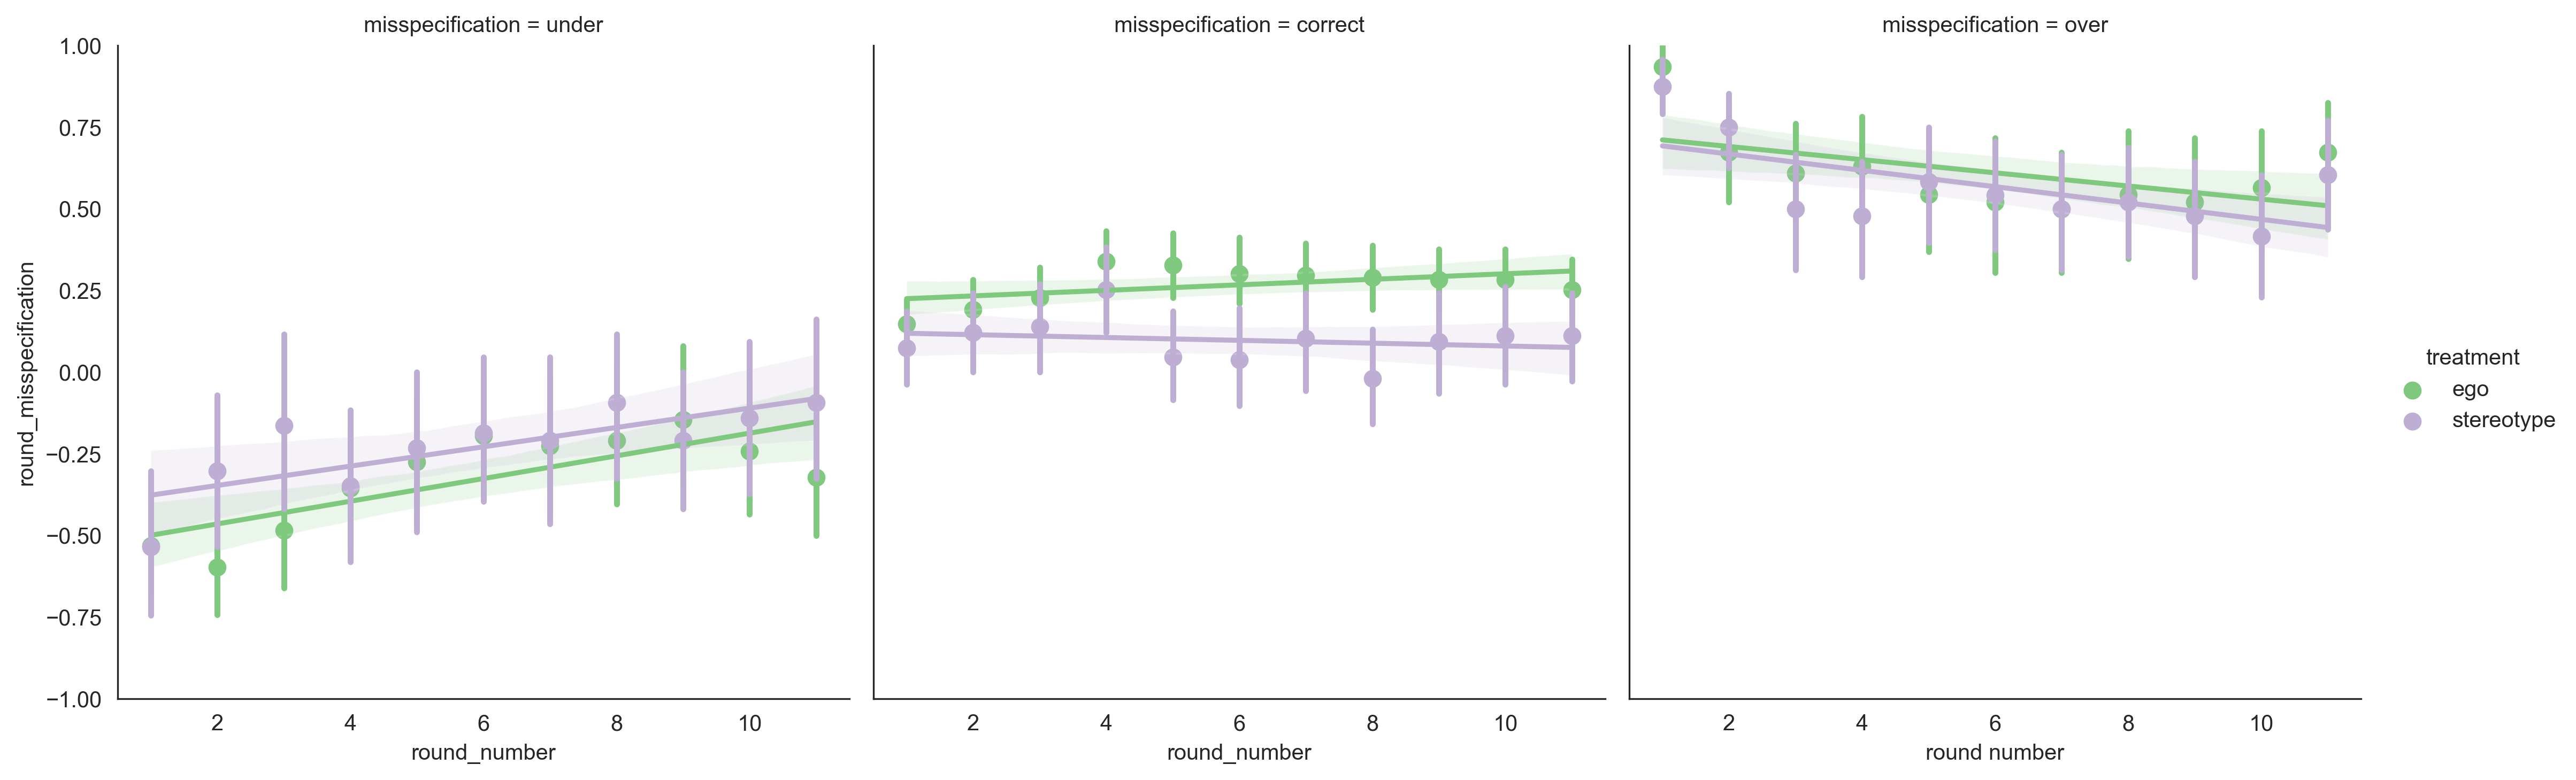
\includegraphics[scale=.5]{misspecification_round_tratment.png}
    \end{figure}
    \action{\hyperlink{misspecificationsroundstypes}{\beamerbutton{Back}}}
\end{frame}

\begin{frame}{Positive Signals v. Negative Signals}
    \label{positivevnegative}
    \begin{figure}
        \centering
        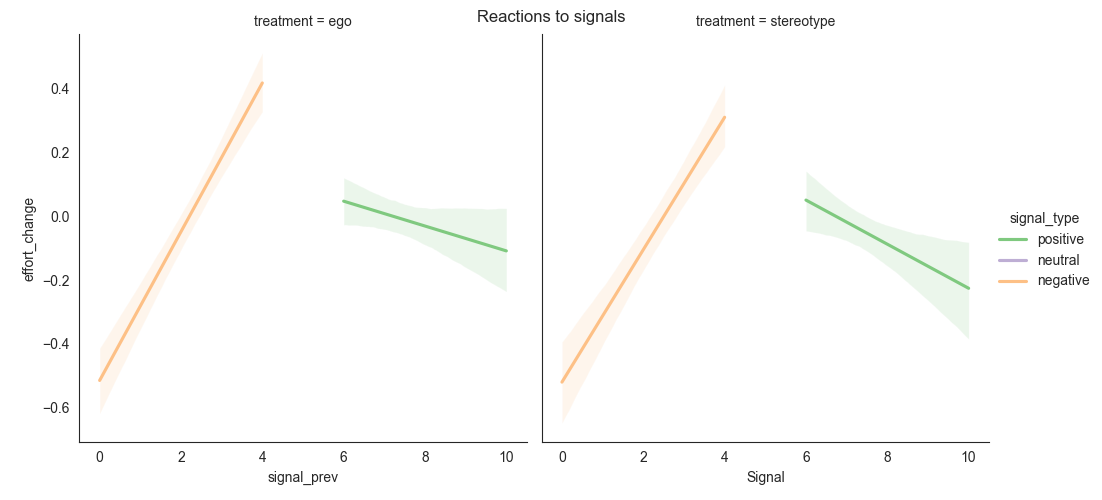
\includegraphics[scale=.5]{signalvalue_effort_change.png}
    \end{figure}
    \action{\hyperlink{goodvbad}{\beamerbutton{Back}}}

\end{frame}

\begin{frame}{Dogmatic v. Switcher}
    \label{pathdistances}
    \begin{figure}
        \centering
        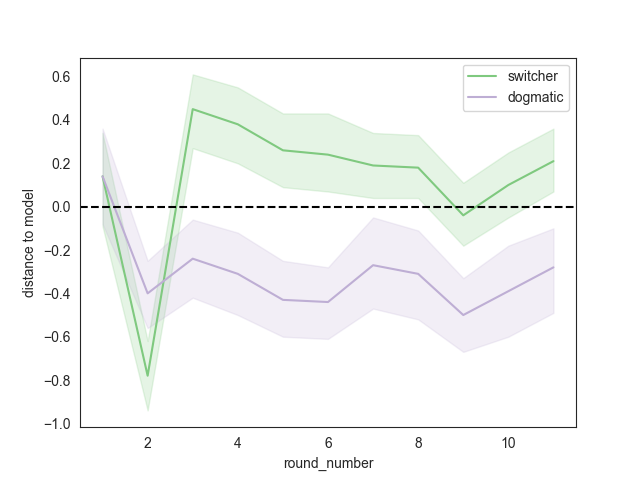
\includegraphics[scale=.5]{distances_switch_dog.png}
    \end{figure}
    \action{\hyperlink{meandistances}{\beamerbutton{Back}}}
\end{frame}

\begin{frame}{Bayesian v. Self-Attribution}
    \begin{figure}
        \centering
        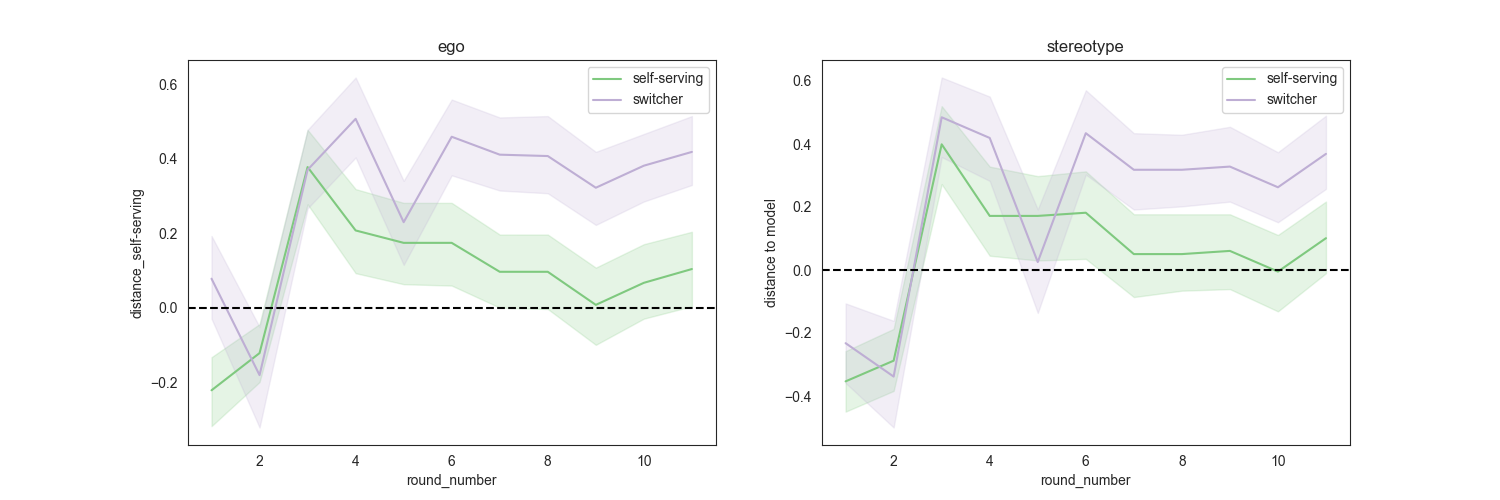
\includegraphics[scale=.5]{distances_bay_ss.png}
    \end{figure}
    \action{\hyperlink{meandistances}{\beamerbutton{Back}}}
\end{frame}


\end{document}
